%
% OEFENINGEN 2009
%
  %\documentstyle[11pt,epsfig]{article}
  %\documentclass[chap,11pt,a4paper]{book}
  %\documentclass[art,11pt,a4paper]{article}
  
%\documentclass[12pt,twoside,a4paper,pdftex,dutch]{article}


%%%%%%%%%%%%%%%%%%%%%%%%%%%%%%
%%                          %%
%%  LaTeX => PS => PDF !!!  %%
%%                          %%
%%%%%%%%%%%%%%%%%%%%%%%%%%%%%%


\documentclass[12pt,twoside,a4paper,dutch]{article}

\hyphenation{Galilei-transformatie Galilei-transformaties Lorentz-transformatie Lorentz-transformaties}

\usepackage[dutch]{babel}
\usepackage{epsf}
\usepackage{axodraw}   
\usepackage{amsfonts}
\usepackage{amssymb}

%
%       Loosen up LaTeX float placement
%
\renewcommand{\textfraction}{0.15}
\renewcommand{\topfraction}{0.85}
\renewcommand{\bottomfraction}{0.65}
\renewcommand{\floatpagefraction}{0.60}

\usepackage{graphicx}
\usepackage{hyperref}


\begin{document}

%%%%%%%%%%%%%%%%%%%%%%%%%%%
%\begin{titlepage}
%\begin{center}
%
\includegraphics[width=\textwidth]{./UvAlogo}\\[3.5cm] 
%% Title
%\HRule \\[0.4cm]
%{ \huge \bfseries Oefeningen Speciale Relativiteitstheorie} \\[0.4cm]
%\HRule \\
%\vfill
%
%% Author and supervisor
%\HRule \\[0.1cm]
%\begin{minipage}{0.4\textwidth}
%\begin{flushleft} \large
%A.P. \textsc{Colijn}
%\end{flushleft}
%\end{minipage}
%\begin{minipage}{0.4\textwidth}
%\begin{flushright} \large
%IoP \textsc{IHEF}
%\end{flushright}
%\end{minipage}
%\HRule \\[0.4cm]
%{\large \today}
%\end{center}
%\end{titlepage}
%%%%%%%%%%%%%%%%%%%%%%%%%%%


\begin{center}
{\Large\textsc{Faculteit der Natuurwetenschappen, \\ Wiskunde en Informatica}}
\\[4cm]
{\Huge\bf Oefeningen \\ Speciale Relativiteitstheorie}
\\[1cm]
{\large dr. A.P. Colijn}
\\[0.1cm]
UvA / NIKHEF
\\[0.1cm]  
Onderzoeksinstituut Hoge Energie Fysica (IHEF) 
\\[6.5cm]
\end{center}

%\begin{figure}[ht]
%	\centering
%		
\includegraphics[width=0.10\textwidth]{logo_uva2.PNG}
%	\label{fig:Uvalogo2}
%\end{figure}
%\begin{center}
%{\Large\textsc{Universiteit van Amsterdam}}
\normalsize

\begin{figure}[ht]
	\centering
		
\includegraphics[width=0.5\textwidth]{oefeningen.pictures/UVA}
	\label{fig:UVA}
\end{figure}
%



\thispagestyle{empty}
\newpage
\thispagestyle{empty}
\newpage
\cleardoublepage

\title{\Huge\bf Oefeningen \\ Speciale Relativiteitstheorie}
\author{\large dr. A.P. Colijn\\[0.1cm]
UvA / NIKHEF\\[0.1cm]  
Onderzoeksinstituut Hoge Energie Fysica (IHEF) \\[0.5cm]
gebaseerd op de syllabus van Prof. S. Bentvelsen\\[0.1cm]
gebaseerd op de syllabus van Prof. J.J. Engelen\\[0.1cm]
met medewerking van \\[0.1cm]
drs. B. Mooij en B. Elsinga BSc\\[1.0cm]
versie 7.0, augustus 2012}

%\begin{figure}[ht]
%	\centering
%		
\includegraphics[width=0.5\textwidth]{UVA}
%	\label{fig:UVA}
%\end{figure}

\date{}
\maketitle 
\thispagestyle{empty}
\cleardoublepage


%table of contents
\pagestyle{plain}
\pagenumbering{roman}
\setcounter{page}{1}
\tableofcontents
\cleardoublepage

% Hoofdtekst
\pagestyle{headings}
\pagenumbering{arabic}
\setcounter{page}{1}

\section{Galileitransformatie}
%%%%%%%%%%%%
\subsection{Twee inertiaalsystemen}
Twee inertiaalstelsels $S$ en $S'$ zijn verbonden door de 
Galileitransformatie :
\begin{eqnarray*}
x' & = & x + 3t \\ 
y' & = & y \\
z' & = & z \\
t' & = & t 
\end{eqnarray*}
\begin{itemize}
\item [a.] In welke richting beweegt $S$ t.o.v. $S'$?
\item [b.] Schrijf de transformatie-formules op voor de 
snelheidscomponenten
$v_{x}$, $v_{y}$, $v_{z}$.
\end{itemize}
In $S$ duwt een kracht $F$ een voorwerp met massa $m$ 
met een versnelling 
$a = 2 $m/s$^{2}$ voort: van snelheid $v = 4$m/s op 
$t = 0$ en $x = 0$, tot snelheid
$v = 10$m/s op $t = 3$s en $x = 21 $m.
\begin{itemize}
\item [c.]
Welke waarden hebben $a, F, x$ en $v $ in $S'$?
\item [d.]
Blijft de formule $v$ = $v(0)$ + $at$ in $S'$ van kracht?
\end{itemize}
Zowel in $S$ als $S'$ kun je de arbeid $W = F\Delta$x en de groei van de 
kinetische energie $\Delta E_{k}$ = $\Delta (\frac{1}{2}mv^{2})$ uitrekenen.
\begin{itemize}
\item [e.]
Is de arbeid die verricht wordt hetzelfde, gezien vanuit $S$ en $S'$?
\item [f.]
Dezelfde vraag voor $\Delta E_{k}$.
\item [g.]
Geldt zowel in $S$ als in $S'$ dat $F\Delta x$ gelijk is aan 
$\Delta (\frac{1}{2}mv^{2})$?
\item [h.]
Omschrijf nu wat het relativiteitsprincipe inhoudt voor 
Galileitransformaties.
\end{itemize}


%%%%%%%%%%%%
\subsection{Tennissen}
 \begin{figure} [h]
 \begin{center}
 \mbox{\epsfxsize=10cm\epsffile{oefeningen.pictures/tennis.eps}}
 \caption{Tennissen}
 \label{f:tennis}
 \end{center}
 \end{figure}
Een satelliet die zich om een bewegende planeet slingert, krijgt
daarvan een extra snelheid mee, ongeveer zoals een tennisbal dat van een
bewegende tennisracket krijgt. $v_{b}$, $v_{e}$ en $v_{0}$ zijn de
begin-, eind- , planeet/tennisracket-snelheid in het co\"ordinatenstelsel
$S$ van de toeschouwer. $S'$ is het co\"ordinatenstelsel dat met de
planeet/tennisracket meebeweegt.
\begin{itemize}
\item [a.]
Wat zijn de begin- en eindsnelheid van de bal in het 
co\"{o}rdinatenstelsel $S'$?
\end{itemize}
Bij de elastische botsing van de bal met het racket is in $S'$
is de snelheid van de bal na de botsing even groot 
als de snelheid voor de botsing.
\begin{itemize}
\item [b.]
Hoe groot is de eindsnelheid van de bal in $S$ in termen 
van $v_{b}$ en $v_{0}$?
\item [c.]
Hoe verandert de kinetische energie $E_{k} = \frac{1}{2}mv^{2}$ van de bal 
in $S$?
\item[d.] 
En in $S'$?
\end{itemize}
Terwijl  de {\it waarden} van grootheden in $S$ en $S'$ kunnen verschillen, 
moeten de formules tussen de  grootheden  wel {\it invariant} zijn. 
\begin{itemize}
\item [e.]
Laat zien dat de formule $\Delta E_{k} =F\Delta x$ zowel in $S$ als in $S'$ 
geldt (het racket werkt met $F = m_{bal}\frac{\Delta v}{\Delta t}$ over een 
afstand $\Delta x = v_{0} \Delta {t}$).
\end{itemize}
%
%\begin{figure} [h]
%\begin{center}
%\mbox{\epsfxsize=3cm\epsffile{oefeningen.pictures/planet.eps}}
%\caption{}
%\label{f:planeet}
%\end{center}
%\end{figure}

%%%%%%%%%%
\subsection{Een paraboolbaan}

% \begin{figure} [h]
% \begin{center}
% \mbox{\epsfxsize=5cm\epsffile{oefeningen.pictures/parabool.eps}}
% \caption{Paraboolbaan}
% \label{f:parabool}
% \end{center}
% \end{figure}

\begin{figure}[ht]
\centering
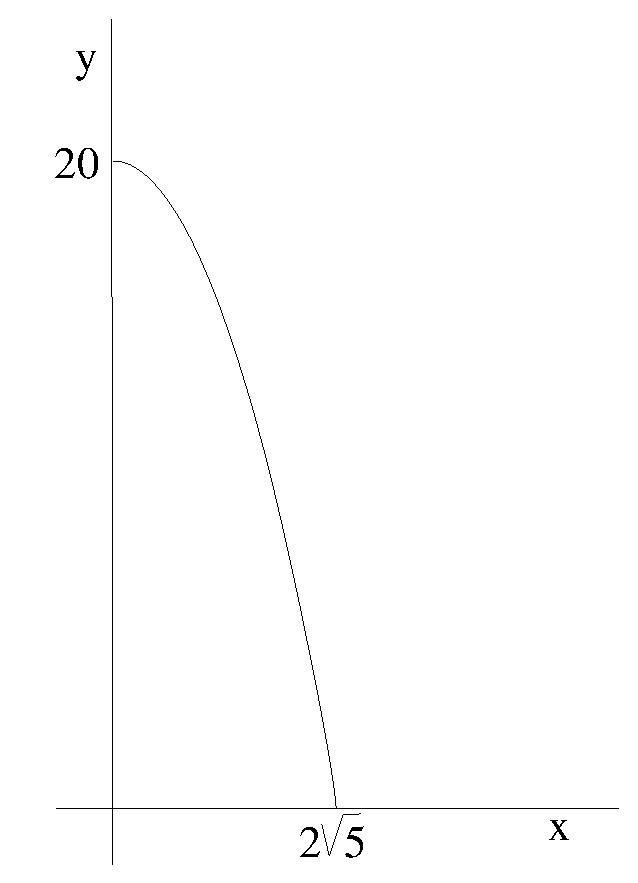
\includegraphics[width=.5\textwidth]{oefeningen.pictures/parabool}
\caption{Paraboolbaan}
\label{f:parabool}
\end{figure}


Gegeven een paraboolbaan (zie figuur \ref{f:parabool}) t.o.v.
co\"{o}rdinatenstelsel $S$:
\begin{displaymath}
y = -x^{2} + 20
\end{displaymath}
Dit is de baan die beschreven wordt door een puntmassa die met een
horizontale beginsnelheid van een 20 meter hoge toren gegooid wordt.
De versnelling van de zwaartekracht is $g = 10$ m/s$^{2}$.
Geef de Galileitransformatie naar stelsel $S'$ zodat de puntmassa t.o.v. dit
stelsel langs een rechte, verticale lijn beweegt.

%%%%%%%%%%%%
\subsection{Versnellende auto}
Als  je  vanuit  een  inertiaalsysteem  een Galileitransformatie uitvoert, 
kom je in een ander inertiaalsysteem.
\begin{itemize}
\item [a.]
Hoe weet je zeker dat je in een inertiaalsysteem bent?
\end{itemize}
Het  interieur van een auto (stelsel $S'$), die versneld door een straat 
(stelsel $S$) rijdt, is g\'{e}\'{e}n  
inertiaalsysteem  en  de transformatie van $S'$ naar $S$ is g\'{e}\'{e}n
Galileitransformatie:    
\begin{eqnarray}
\label{v:auto}
x = x' \pm \frac{1}{2} at^{2}  \\
y = y'  \\
z = z'
\end{eqnarray}

\begin{itemize}
\item [b.]
Moet je in formule \ref{v:auto} het plus- of het minteken nemen?
\item [c.]
Een bal die je binnen in de auto op $t = 0$ loslaat, heeft dan $v = 0$ en 
$v' = 0$.\\
In welk stelsel, $S$ of $S'$ geldt tijdens de val van de bal 
$v_{x} = 0$? 
\item [d.]
Leidt nu uit de transformatieformules  af  hoe de snelheid in $S'$
zich ontwikkelt.
\item [e.]
In  $S'$ is er een versnelling $a_{x}$, en voel je dus
een `kracht' $F_{x }= ma_{x}$.\\
Hoe groot is de kracht en in welke richting werkt de kracht?
\end{itemize}

%%%%%%%%%%%%%
\subsection {Michelson-Morley voor geluid}
V\'{o}\'{o}r  de komst van de speciale relativiteitstheorie veronderstelde 
men dat de lichtsnelheid een vaste  waarde  had in \'{e}\'{e}n 
bepaald inertiaalsysteem (de `ether') en dat de lichtsnelheid in 
andere systemen  via  een  Galileitransformatie kon worden afgeleid. 
Deze veronderstelling bleek niet houdbaar  (zie  o.a.  het  
Michelson-Morley experiment), maar hij geldt {\it wel} voor geluid. 
Vandaar deze opgave, als contrast met de gang van zaken voor licht.

Geluid  heeft  een  vaste  snelheid  t.o.v.  zijn  medium  
(de  lucht,  stelsel $S$),  nl. 
$c_{g} = 1/\sqrt{\rho\kappa}$
waar $\rho$ de dichtheid en $\kappa$ de `compressibiliteit' van de lucht zijn.

% \begin{figure} [h]
% \begin{center}
% \mbox{\epsfxsize=10cm\epsffile{oefeningen.pictures/wind.eps}}
% \end{center}
% \caption{Michelson en Morley voor geluid}
% \label{f:oef1-6}
% \end{figure}

\begin{figure}[ht]
\centering
%\mbox{\epsfxsize=10cm\epsffile{oefeningen.pictures/wind.eps}}
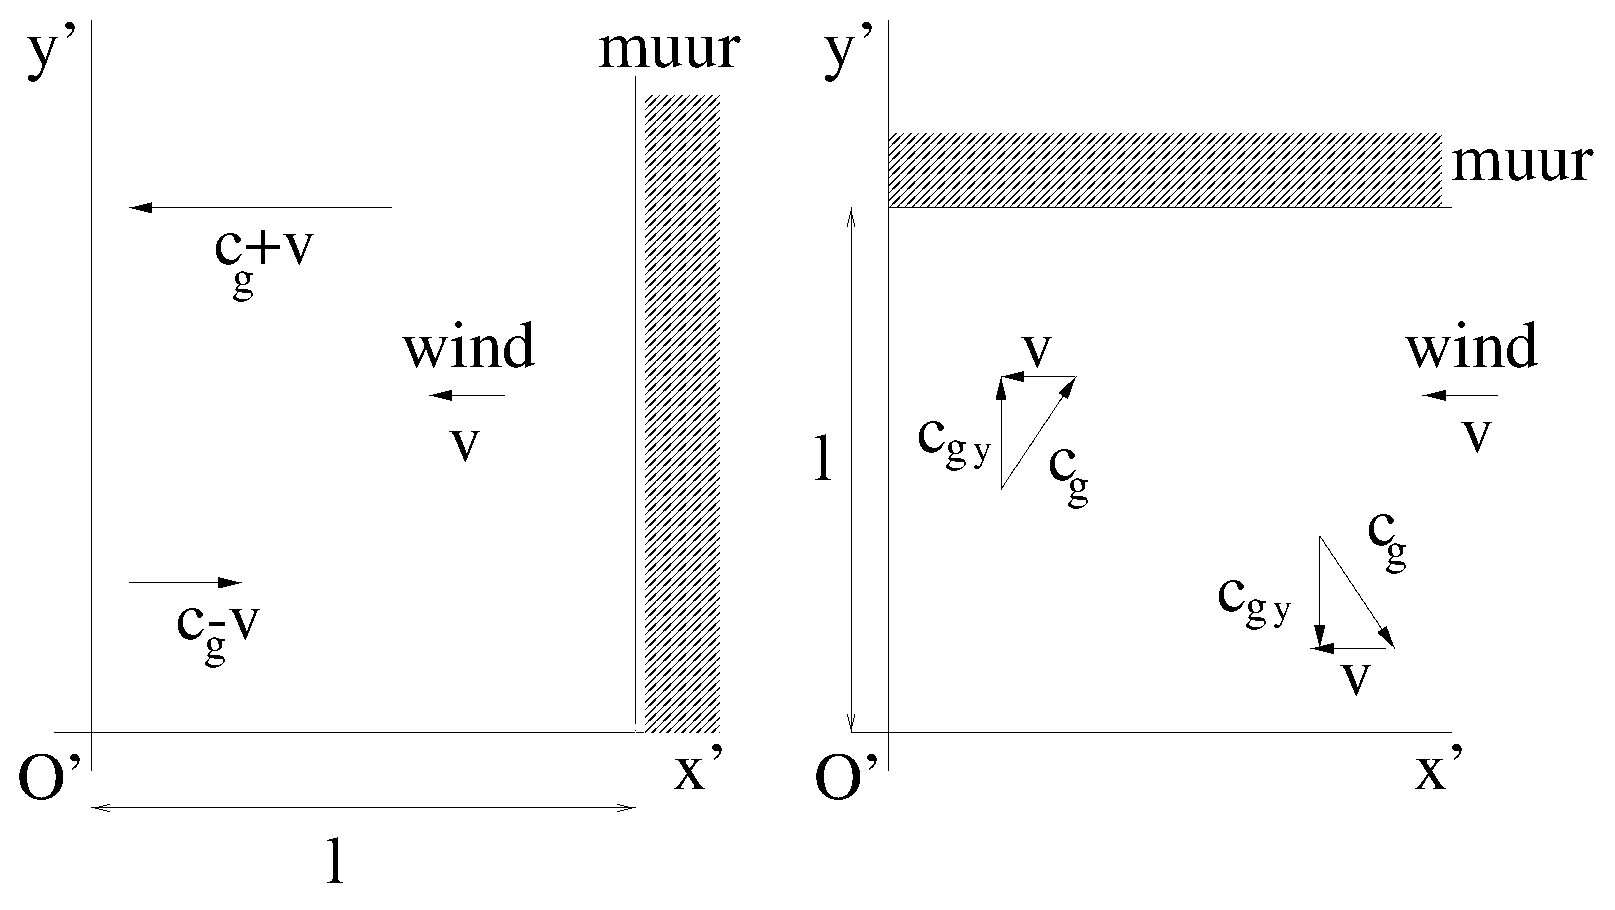
\includegraphics[width=1.0\textwidth]{oefeningen.pictures/wind}
\caption{Michelson en Morley voor geluid}
\label{f:oef1-6}
\end{figure}


Als  in je eigen stelsel ($S'$) de wind je tegemoet blaast met snelheid 
$v$ (of als je met snelheid $v$  naar  voren  beweegt),  is  de  
geluidssnelheid  in  $S'$  volgens de Galileitransformatie gelijk aan 
$c_{g}-v$.\\
We kunnen deze beweging t.o.v. het medium aantonen door de reistijden van het
geluid te meten langs gelijke trajecten in onderling loodrechte
richtingen (de $x'$- en $y'$-as van $S'$).


\begin{itemize}
\item [a.]
  Bereken na hoeveel tijd je de echo uit de $x$-richting en 
  uit de $y$-richting hoort als het windstil is. Is er verschil? 
\end{itemize}
Nu  waait  er  wel  wind,  van  rechts, zoals aangegeven in figuur
\ref{f:oef1-6},
Het geluid moet dan in $S$ schuin naar rechts lopen, om in $S'$ langs 
de $y'$-as heen er weer te gaan (zie figuur \ref{f:oef1-6} rechts).
\begin{itemize}
\item [b.]
Hoeveel tijd kost het nu voor je de echo uit de $x$-richting hoort?
\item [c.]
  En uit de $y$-richting?
\item [d.]
Hoe zou je dus, als je de wind niet zou kunnen voelen of zien, toch kunnen 
constateren dat hij waait? (Neem bijv. $l = 340$m; $v = 20$ m/s en $c_{g} = 340$ m/s)
\end{itemize}

         %bijgewerkt 22:32-15/01/2009
\section{Tijddilatatie en lengtecontractie}



\subsection{Einstein puzzel}
Einstein, als jongen van 16, vroeg zich het volgende af: een hardloopster
ziet zichzelf in een spiegel die zij in haar hand houdt, een armlengte
voor haar gezicht. Als zij nu met bijna de snelheid van het licht
rent, zal ze zichzelf dan nog steeds in de spiegel zien? Analyseer deze
vraag aan de hand van het relativiteitsprinciepe.

\subsection{Tijddilatatie}
Een waarnemer D heeft een lichtklok en een polshorloge, beide in rust
ten opzichte van hemzelf.  Een andere waarnemer E beweegt ten opzichte
van waarnemer D, en kan de lichtklok en polshorloge van D bekijken.
We vragen ons af of het mogelijk is dat waarnemer D zijn twee klokken
gelijk ziet lopen, terwijl waarnemer E observeert dat de klokken niet
gelijk lopen. Laat met behulp van een gedachtenexperiment zien dat dit
onmogelijk is \textit{(hint: stel voor dat de beide klokken van D bij elke tik
een gaatje prikken in een tape)}.


\subsection{Einsteins \textit{Gedankenexperiment}}
Als werknemer bij een patentburo in Bazel zag Einstein vanaf zijn
werkkamer de klok van de kerktoren. Op een bepaald moment stond de
klok op precies 3~uur.  Hij stelde zich voor dat het licht, dat
weerkaatst wordt vanaf de klok en het `beeld' van de klok met zich
draagt, met een snelheid van 300.000 km/s de ruimte in suist. Hij vroeg
zich af hoe je de klok ziet lopen als je met dit licht zou kunnen
meereizen.
\begin{itemize}
\item [a.] Hoe verloopt de tijd voor een (hypothetische) waarnemer die met de snelheid van het licht reist?
\end{itemize}

\subsection{Afstanden}
In het ruststelsel van de aarde is de afstand tussen Amsterdam en New
York ongeveer 6000 km (5.877 km om precies te zijn). Met hoeveel wordt
de afstand tussen de steden verkort, geobserveerd vanuit een
vliegtuig (1000 km/uur)? Of door de International Space Station (8
km/s)? Of door een kosmisch deeltje dat met een snelheid van 0,9$c$
reist?

%%%%%%%
\subsection{Muon}
Een muon ($\mu$-deeltje) is een instabiel elementair deeltje, dat in 
{\it rust} een gemiddelde levensduur $\tau_{0} = 2,2 \cdot 10^{-6}$ s  heeft.  
Veronderstel dat een gegeven muon in een laboratorium (stelsel $S$) een 
buis met een lengte $l =600$ m kan doorlopen voordat het vervalt. 
\begin{itemize}
\item [a.]
  Druk de levensduur $\tau$ van een muon in het laboratorium uit in zijn 
snelheid $v$.
\item [b.]
  Gebruik het gegeven dat het muon binnen $\tau$ s de buis van $600 $ m kan 
doorlopen om $v$ te berekenen. 
\item [c.]
  Hoe lang was volgens het muon zelf de buis die aan hem voorbij schoot? 
\item [d.]
  Leeft het muon volgens zichzelf lang genoeg om de Lorentz-gecontraheerde 
buis te passeren?
\end{itemize}

%%%%%%%%
\subsection{Neutron}
De gemiddelde levensduur van een neutron is 15 minuten 
(daarna vervalt hij in een proton, elektron en antineutrino). 
Toch zijn er neutronen die vanuit de zon de aarde bereiken (afstand 
$\approx 1,5 \cdot 10^{11}$  m). 
  Met welke snelheid moeten die minstens door de zon zijn uitgestoten?

%%%%%%%%%%
\subsection{Astronaut}
Een astronaut wil binnen \'{e}\'{e}n jaar (volgens zijn eigen tijdrekening) 
een ster die op een afstand van 5 lichtjaren staat bereiken. 
Neem als lengte-eenheid lichtjaar en als tijdseenheid jaar.
\begin{itemize}
\item [a.]
Welke waarde heeft de lichtsnelheid $c$ in deze eenheden?
\item [b.]
Welke snelheid moet zijn ruimteschip dan hebben?
\item [c.]
Hoelang duurt de reis volgens de aardse tijdrekening?
\end{itemize}

%%%%%%%%%
\subsection{Bewegend voorwerp}
\begin{itemize}
\item [a.]
  Hoe verandert door de Lorentz-contractie de vorm en de inhoud van een 
bewegend volume?
\item [b.]
  Hoe verandert de dichtheid van een bewegend voorwerp?
\end{itemize}

      %bijgewerkt 22:39-15/01/2009
\chapter{Lorentztransformatie}
\vspace{-1cm}\begin{flushright}
{\it `Its not that I am smart, \\it's just that I stay with the problem longer'}\\ A. Einstein
\end{flushright}

Het tweede postulaat zoals geformuleerd in het voorgaande hoofdstuk is
duidelijk in tegenspraak met de Galileitransformatie en het is nu onze
taak een transformatie te vinden (het eerste postulaat zegt in feite
dat die er moet zijn) die in overeenstemming is met het tweede
postulaat.  Deze transformatie is in 1905 door Einstein gevonden en is
bekend geworden onder de naam Lorentztransformatie.  De afleiding
ervan is wiskundig gezien zeer eenvoudig, maar vereist, zoals we
zullen zien, nogal wat hersengymnastiek.

\section{Invariante interval}
We hebben gezien dat in de drie-dimensionale ruimte de co\"ordinaten van
twee punten $\vec{p}_1$ en $\vec{p}_2$ voor verschillende waarnemers,
waarvoor de onderlinge referentiesystemen zijn getransleerd, anders
zijn. Ze zijn het in deze drie-dimensionale ruimte wel eens over de
afstand tussen deze twee punten; dit is de invariant $\Delta r$.

We willen nu een dergelijke grootheid vinden voor een paar van `gebeurtenissen', een lengte in
de 3+1 dimensionele ruimte-tijd. Beschouw hiervoor persoon
$A$ die zich in de oorsprong van co\"{o}rdinaten-stelsel $S$ bevindt en
een persoon $B$ in de oorsprong van $S^{'}$.  $S^{'}$ beweegt
t.o.v. $S$ in de positieve $x$-richting met snelheid $v$.  Op $t=0$
valt de oorsprong van $S$ samen met die van $S^{'}$, d.w.z. vallen $A$
en $B$ samen.  Op $t=0$ ontsteekt $A$ heel eventjes een lampje
waardoor zich een bolvormige lichtgolf gaat uitbreiden.  $A$ bevindt
zich in het middelpunt van de bolvormige golf.  Een bol met straal $R$
en de oorsprong van het co\"{o}rdinatenstelsel als middelpunt wordt
beschreven door de formule :
\begin{displaymath}
x^{2} + y^{2} + z^{2} = R^{2}(t)
\end{displaymath}

% \begin{figure}[h]
% \begin{center}
% \mbox{\epsfxsize=8cm\epsffile{syllabus.pictures/spheres.eps}}
% \caption{Bolvormige lichtgolf}
% \label{f:lorentz1}
% \end{center}
% \end{figure}

\begin{figure}[ht]
\centering
%\includegraphics[width=1.00\textwidth]{syllabus.pictures/bolgolf}
\epsfig{file=bolgolf.pdf, width=\textwidth}
\caption{{\sl Bolvormige lichtgolf}}
\label{f:lorentz1}
\end{figure}


Voor een lichtgolf die zich uitbreidt met snelheid $c$ geldt na een tijd $t$: 
$R = ct$ en dus :
\begin{displaymath}
x^{2} + y^{2} + z^{2} = c^{2}t^{2}
\end{displaymath}
oftewel
\begin{equation}
\label{v:lorentz0a}
c^2 t^2 - x^{2} - y^{2} - z^{2} = 0
\end{equation}
Precies dezelfde redenering kunnen we echter volgen voor persoon $B$.
Ook $B$ denkt zich in het midden van de bolvormige lichtgolf te bevinden, het 
tweede postulaat zegt immers dat ook voor B het licht zich met snelheid $c$ 
uitbreidt.
Voor $B$, dus t.o.v. $S^{'}$, geldt nu geheel in analogie met hierboven :
\begin{displaymath}
x'^{2} + y'^{2} + z'^{2} = c^{2}t'^{2}
\end{displaymath}
oftewel
\begin{equation}
\label{v:lorentz0b}
c t'^2 - x'^{2} - y'^{2} - z'^{2} = 0
\end{equation}
In ons specifieke voorbeeld (beweging in de $x$-richting), geldt 
$(x \neq x^{'},$\newline $y = y^{'}, z = z^{'})$ dus moeten we wel concluderen 
$t \neq t^{'}$ (Aftrekken van \ref{v:lorentz0a} en \ref{v:lorentz0b} levert
$x^{2} - x'^{2} = c^{2}(t^{2} - t'^{2})$ en dus $t^{2} - t'^{2} \neq 0$) .
We komen al snel tot de conclusie dat de tijd voor $B$ anders 
verloopt dan voor $A$.\\
Bij elk referentiestelsel hoort niet alleen een eigen plaatsmeting maar 
ook een eigen tijdmeting.
Hoe plaats en tijd van een bepaald natuurkundig verschijnsel zoals geldend 
in $S$ worden uitgedrukt in plaats en tijd van hetzelfde verschijnsel 
t.o.v. $S^{'}$ wordt gegeven door de Lorentztransformatie.

In elk geval weten we al (zie boven) dat zal moeten gelden:
\begin{equation}
\label{v:lorentz1}
c^2 t'^2 - x'^{^{2}} - y'^{^{2}} - z'^{^{2}} = c^2 t^2 - x^{2} - y^{2} - z^{2} 
\end{equation}
We zeggen dat de grootheid $c^2 t^2 - x^{2} - y^{2} - z^{2}$
{\sl invariant} is onder Lorentztransformaties. 

Iets algemener kunnen we twee gebeurtenissen A en B in het stelsel $S$ beschouwen, met onderling tijdsverschil $\Delta t$ en
ruimteverschillen $(\Delta x,\Delta y, \Delta z)$. We hebben laten zien dat de afstand tussen deze twee gebeurtenissen,
gedefinieerd als 
\begin{eqnarray}
(\Delta s)^2 & \equiv & (c \Delta t)^2 - (\Delta r)^2 \\
             & \equiv & (c \Delta t)^2 - (\Delta x)^2 - (\Delta y)^2 - (\Delta z)^2
\end{eqnarray}
{\it invariant} is onder het relativiteitsprincipe van Einstein.
Dit invariante interval staat centraal in de speciale relativiteitstheorie.

\subsection{Nogmaals de lichtklok}
In paragraaf~\ref{s:lichtklok} hebben we de lichtklok
ge\"introduceerd. In het referentiesysteem van D waarin de klok stil staat, tikte de klok met
tikken van $(c\Delta t)=1$ m (elke 3.3 ns), en de afgelegde afstand in de $x$-richting tussen twee tikken is $\Delta
x=0$. Het invariante interval tussen twee tikken wordt daarmee $(\Delta
s)^2 = (c \Delta t)^2-(\Delta x)^2 = 1 $m$^2$. 

In het referentiestelsel
van E is $c \Delta t' = \gamma$(1 m) en de afgelegde afstand afstand in $x$ tussen twee tikken wordt
gegeven door de snelheid $v$ te vermenigvuldigen met de het tijdsverschil $\Delta t'$, $\Delta x' = \gamma v$(1 m)$/c$. Het
interval in E's referentiesysteem wordt hiermee $(\Delta s')^2
=\gamma^2(1-v^2/c^2)$(1 m$^2$). Omdat geldt dat $\gamma\equiv
1/\sqrt{(1-v^2/c^2)}$, wordt het interval hiermee $(\Delta s')^2 =
(\Delta s)^2 = 1$ m$^2$. We hebben laten zien dat het interval
dezelfde waarde heeft voor waarnemer D en waarnemer E. Voor elke
andere waarnemer die in een referentiesysteem zit, geldt dat hij
andere tijdverschillen meet, en andere ruimte afstanden vindt. Maar het
interval $(\Delta s)^2$ blijft altijd 1 m$^2$.

\section{De eigentijd en eigenlengte}
De {\sl eigentijd} $\Delta \tau$ tussen twee gebeurtenissen is het
tijdsinterval zoals waargenomen in een co\"ordinatenstelsel waarin de
twee gebeurtenissen op dezelfde positie plaatsvinden. Dit is niet in
alle gevallen mogelijk.  Zoals in bovenstaand voorbeeld duidelijk is
gemaakt, is het invariante interval tussen twee gebeurtenissen $c$
maal de eigentijd, of $c\Delta \tau = \sqrt{(\Delta s)^2}$. De
eigentijd is het tijdsinterval in het co\"ordinatenstelsel van D, het
stelsel waarin de lichtklok stil staat. De eigentijd is de tijd zoals
die verloopt voor de waarnemer zelf; het is zijn {\it eigen} tijd.


 Als het interval positief is, is er altijd een co\"ordinatenstelsel te
vinden waarin de positie van de gebeurtenissen hetzelfde is. Dit omdat
een positief interval betekent $|c \Delta t | > | \Delta r|$, dus een
referentiesysteem dat beweegt met een snelheid $\vec{v}=(\Delta
\vec{r})/(\Delta t)$ transformeert  de gebeurtenissen naar hetzelfde punt. En 
de  snelheid is kleiner dan die van het licht. 

Als het interval tussen twee gebeurtenissen kleiner is dan nul, d.w.z.
$(\Delta s)^2 < 0$, is het nog steeds een invariant. Maar er kan in dit
geval geen co\"ordinatenstelsel gevonden worden waarin beide
gebeurtenissen op dezelfde positie plaatsvinden. Dit
co\"ordinatenstelsel is er niet - het zou sneller dan met de lichtsnelheid
moeten bewegen ten opzichte van het stelsel van de twee
gebeurtenissen. Soms wordt hiervoor de {\it eigenlengte} ge\"introduceerd, $\Delta \lambda$, als
de ruimtelijke afstand tussen twee gebeurtenissen in een referentiesysteem waarin de gebeurtenissen
gelijktijdig plaatsvinden. Dit kan alleen als het interval negatief is, en de eigenlengte wordt
dan $\Delta \lambda = \sqrt{|(\Delta s)^2|}$. 

Het interval $(\Delta s)^2$ kan natuurlijk ook precies gelijk zijn
aan nul. Dit is het geval wanneer $(c \Delta t)^2 = (\Delta r)^2$,
met andere woorden, wanneer de wereldlijn overeenkomt met die van het
licht. Omdat de lichtsnelheid in elk co\"ordinatenstelsel dezelfde is,
is dit interval weer gelijk aan nul in elk co\"ordinatenstelsel.

Intervallen $(\Delta s)^2=0$ noemen we {\sl `lichtachtig'}. Intervallen $(\Delta s)^2>0$ noemen we {\sl `tijdachtig'} en
intervallen $(\Delta s)^2< 0$ noemen we {\sl `ruimteachtig'}. Deze intervallen hebben verschillende eigenschappen
met betrekking tot causaliteit; we komen hier op terug.



\section{De Lorentztransformatie, een eenvoudige afleiding}
We defini\"{e}ren co\"{o}rdinatenstelsels $S$ en $S^{'}$ weer als voorheen:
$S^{'}$ beweegt t.o.v. $S$ met constante snelheid $v$ in de positieve 
$x$-richting.
Op $t = t^{'} = 0$ valt de oorsprong van $S$ samen met die van $S^{'}$.
Een lichtflits, uitgezonden in de positieve $x$-richting, bevindt zich op 
plaats $x = ct$, d.w.z. $x - ct = 0$.
T.o.v. $S^{'}$ geldt $x' - ct^{'} = 0$ (zelfde $c$, tweede postulaat!).
Aan beide vergelijkingen wordt voldaan als geldt:
\begin{equation}
x^{'} - ct^{'} = \lambda (x - ct)
\end{equation}
waar $\lambda$ een constante is die we nog moeten bepalen.
We kunnen uiteraard dezelfde redenering volgen voor een lichtflits die wordt 
uitgezonden in de negatieve $x$-richting.
Dan vinden we dat moet gelden:
\begin{equation}
\label{v:lorentz2}
x^{'} + ct^{'} = \mu (x + ct)
\end{equation}
Ook $\mu$ is een nog nader te bepalen constante.
Optellen resp. aftrekken van \ref{v:lorentz1} en \ref{v:lorentz2} levert:
\begin{displaymath}
ct^{'} = \frac{\lambda + \mu}{2} ct - \frac{\lambda - \mu}{2} x \\
\end{displaymath}
\begin{displaymath}
x^{'} = \frac{\lambda + \mu}{2} x - \frac{\lambda - \mu}{2} ct 
\end{displaymath}
We defini\"{e}ren twee nieuwe constanten, $a = \frac{\lambda + \mu}{2}$
en $b = \frac{\lambda - \mu}{2}$ en verkrijgen de overzichtelijke 
vergelijkingen:
\begin{equation}
\label{v:lorentz4}
ct^{'} = act - bx
\end{equation}
\begin{equation}
\label{v:lorentz3}
x^{'} = ax - bct
\end{equation}
waar we nog steeds als taak hebben om $a$ en $b$ te bepalen (d.w.z. uit te 
drukken in $v$, de parameter die de transformatie defini\"{e}ert.)

Voor de oorsprong van $S^{'}$ geldt t.o.v. $S$:
\begin{displaymath}
x = vt
\end{displaymath}
en t.o.v. $S^{'}$ uiteraard:
\begin{displaymath}
x^{'} = 0
\end{displaymath}
Invullen in \ref{v:lorentz3} levert dan dat moet gelden:
\begin{equation}
\label{v:lorentz5}
v = \frac{b}{a}c
\end{equation}

% \begin{figure}
% \begin{center}
% \mbox{\epsfxsize=8cm\epsffile{syllabus.pictures/ruler.eps}}
% \caption{Meetlat}
% \label{f:lorentz2}
% \end{center}
% \end{figure}

\begin{figure}[ht]
\centering
\epsfig{file=ruler.pdf, width=0.5\textwidth}
%\includegraphics[width=.5\textwidth]{syllabus.pictures/ruler}
\caption{Meetlat}
\label{f:lorentz2}
\end{figure}


Nu gebruiken we het relativiteitsprincipe in de volgende redenering: 
een meetlat die langs de $x^{'}$-as ligt, in rust t.o.v. $S^{'}$, 
heeft, gezien vanuit $S$ dezelfde lengte als diezelfde meetlat, gelegen 
langs de $x$-as, in rust t.o.v. $S$, gezien vanuit $S^{'}$!
\begin{itemize}
\item \underline{Observatie 1} \\
Op een zekere tijd $t$ in $S$ kunnen we dus de lengte van de meetlat 
t.o.v. $S^{'}$ bepalen, bijvoorbeeld op \underline{$t = 0$}.
We vinden dan met behulp van \ref{v:lorentz3}:
\begin{displaymath}
x^{'} = ax
\end{displaymath}
\item \underline{Observatie 2} \\
Omgekeerd vinden we op \underline{$t^{'} = 0$}, m.b.v. \ref{v:lorentz3} en 
\ref{v:lorentz4} en gebruikmakend van \ref{v:lorentz5}:
\begin{displaymath}
x^{'} = a(1 - \frac{v^{2}}{c^{2}})x
\end{displaymath}
\end{itemize}
Wanneer we zeggen dat de lengte van de meetlat $l_0$ is, dan bedoelen we: 
de lengte is $l_{0}$ in het systeem waarin de meetlat in rust is.
Observatie 1 (meetlat in rust in  $S^{'}$ gefotografeerd vanuit $S$) leert dan:
\begin{displaymath}
l_{0} = al
\end{displaymath}
waar $l$ dus de lengte t.o.v. $S$ is, d.w.z. ten opzichte van het 
co\"{o}rdinatenstelsel waarin de lat beweegt.
Observatie 2 ($S$ gefotografeerd vanuit $S^{'}$) levert op:
\begin{displaymath}
l = a(1-\frac{v^{2}}{c^{2}})l_{0}
\end{displaymath}
Het combineren van deze resultaten levert dan het volgende resultaat op:
\begin{displaymath}
a = \frac{1}{\sqrt{1-\frac{v^{2}}{c^{2}}}}
\end{displaymath}
Degenen die achterdochtig worden van deze nogal veel woorden kostende 
afleiding vinden de volgende beschouwing misschien eleganter.\\
We pikken de afleiding op na formule \ref{v:lorentz5} en schrijven 
\ref{v:lorentz3} en \ref{v:lorentz4} als :
\begin{equation}
\label{v:lorentz7}
ct^{'} = a(ct - \frac{v}{c}x)
\end{equation}
\begin{equation}
\label{v:lorentz6}
x^{'} = a(x - vt)
\end{equation}
Bovenstaande transformatie geldt als $S^{'}$ beweegt in de positieve 
$x$-richting, dus met snelheid $+v$, t.o.v. $S$.
Maar we kunnen ook $S^{'}$ als rustsysteem kiezen en $S$ als het bewegende 
systeem zien dat t.o.v. $S^{'}$ naar links beweegt, d.w.z. met snelheid $-v$.
De {\sl inverse} transformatie wordt dan onmiddellijk uit de bovenstaande 
verkregen door `accenten te verwisselen' (de accenten slaan immers op het 
bewegende systeem en die rol wordt nu 
overgenomen door $S$) en door $v$ te vervangen door $-v$. 
Dit levert:
\begin{equation}
ct = a(ct^{'} + \frac{v}{c}x^{'})
\label{v:lorentz9}
\end{equation}
\begin{equation}
\label{v:lorentz8}
x = a(x^{'} + vt^{'})
\end{equation}
(Merk op dat deze redenering alleen correct is als $a$ ongevoelig is voor 
het teken van $v$. 
Gelukkig blijkt dat zo te zijn volgens het eerste postulaat.)
Indien we \ref{v:lorentz8} en \ref{v:lorentz9} gebruiken om $t^{'}$ in $t$ 
en $x$ uit te drukken en het resultaat vervolgens vergelijken met 
\ref{v:lorentz7} vinden we 
\begin{displaymath}
a = \frac{1}{\sqrt{1 - \frac{v^{2}}{c^{2}}}}
\end{displaymath}
Aldus hebben we de Lorentztransformatie gevonden:
\begin{displaymath}
ct^{'} = \frac{ct - x \frac{v}{c}}{\sqrt{1 - \frac{v^{2}}{c^{2}}}}
\end{displaymath}
\begin{displaymath}
x^{'} = \frac{x - vt}{\sqrt{1 - \frac{v^{2}}{c^{2}}}}
\end{displaymath}
In ons specifieke geval, relatieve beweging langs de $x$-as, geldt verder
\begin{displaymath}
y^{'} = y
\end{displaymath}
\begin{displaymath}
z^{'} = z
\end{displaymath}
Ga nu na dat formule \ref{v:lorentz1} inderdaad klopt, dat wil zeggen, dat het inderdaad het `invariante interval' $(\Delta s)^2$ invariant laat! Samenvattend:
\begin{quote}
Lorentztransformaties verbinden, net als Galileitransformaties,
inertiaalsystemen op een manier die in overeenstemming is met het
relativiteitsprincipe en het lichtpostulaat. In tegenstelling tot
Galileitransformaties laten ze de lichtsnelheid invariant. Hiermee
zijn ze in overeenstemming met de Maxwell-theorie van het
elektromagnetisme.
\end{quote}

\subsection{Notatie}
We hadden al ingevoerd dat 
\begin{eqnarray}
\beta & = & \frac{v}{c} \\
\gamma & = & \frac{1}{\sqrt{1-\beta^2}}
\end{eqnarray}
De Lorentztransformatie langs de $x$-as wordt hiermee geschreven als:
\begin{eqnarray}
\label{v:lorentz11}
ct' &  = & \gamma (ct - \beta x) \\ \label{v:lorentz10}
x'  &  = & \gamma (x -  \beta ct)\\
y'  & = & y \\
z' & = & z 
\end{eqnarray}
oftewel in matrix vorm\footnote{Voor een overzicht van matrix algebra wordt u doorverwezen naar
de cursus lineare algebra. Kortweg geldt dat een kolom-vector vermenigvuldigd met een matrix een nieuwe kolom-vector oplevert volgens de regel
\[
\left( \begin{array}{c} y_0 \\ y_1 \\ y_2 \\ y_3 \end{array} \right) =
\left( \begin{array}{cccc} a_{00} & a_{01} & a_{02} & a_{03} \\ 
                           a_{10} & a_{11} & a_{12} & a_{13} \\ 
                           a_{20} & a_{21} & a_{22} & a_{23} \\ 
                           a_{30} & a_{31} & a_{32} & a_{33} \end{array} \right) 
\left( \begin{array}{c} x_0 \\ x_1 \\ x_2 \\ x_3 \end{array} \right) =
\left( \begin{array}{c} a_{00} x_0 + a_{01} x_1 + a_{02} x_2 + a_{03} x_3 \\ 
                        a_{10} x_0 + a_{11} x_1 + a_{12} x_2 + a_{13} x_3 \\ 
                        a_{20} x_0 + a_{21} x_1 + a_{22} x_2 + a_{23} x_3 \\ 
                        a_{30} x_0 + a_{31} x_1 + a_{32} x_2 + a_{33} x_3  \end{array} \right). 
\]}.
\begin{equation}
\left( \begin{array}{c} ct' \\ x' \\ y' \\ z' \end{array} \right) =
\left( \begin{array}{cccc} \gamma & -\gamma \beta & 0 & 0  \\ -\gamma\beta & \gamma & 0 & 0  \\ 0 & 0 & 1 & 0  \\ 0 & 0 & 0 & 1 
\end{array} \right) 
\left( \begin{array}{c} ct \\ x \\ y \\ z \end{array} \right) 
\end{equation}
De inverse Lorentztransformatie wordt dan 
\begin{equation}\label{v:lorentz12}
\left( \begin{array}{c} ct \\ x \\ y \\ z \end{array} \right) =
\left( \begin{array}{cccc} \gamma & \gamma \beta & 0 & 0  \\ \gamma\beta & \gamma & 0 & 0  \\ 0 & 0 & 1 & 0  \\ 0 & 0 & 0 & 1 
\end{array} \right) 
\left( \begin{array}{c} ct' \\ x' \\ y' \\ z' \end{array} \right) 
\end{equation}
De ruimte-tijd symmetrie, d.w.z. de verwevenheid van $x$ en $ct$, de 
volstrekt gelijkwaardige rol van beide grootheden, is in deze notatie heel 
duidelijk.

\section{Lorentztransformaties}
De Lorentztransformaties (LT) zijn belangrijk en verdienen een
discussie. De LT transformeren de afstanden $(c\Delta t, \Delta x,
\Delta y, \Delta z)$ tussen de co\"ordinaten van twee gebeurtenissen in
een co\"ordinatenstelsel naar de afstanden $(c\Delta t', \Delta x',$ $
\Delta y', \Delta z')$ in een ander co\"ordinatenstelsel. Het betekent
dat als de LT direct op de co\"ordinaten van \'e\'en gebeurtenis
toegepast worden, impliciet de andere gebeurtenis op co\"ordinaten
$(0,0,0,0)$ in beide stelsels wordt genomen. De transformaties waarbij
de snelheid van een co\"ordinatensysteem anders wordt, noemen we een
{\it boost}. Deze boost-transformaties vormen het hart van de speciale
relativiteitstheorie.

We kunnen eenvoudig de consistentie van de LT laten zien door eerst een
co\"ordinatensysteem te transformeren met snelheid $v$, en vervolgens
weer terug te transformeren met snelheid $-v$. We zullen uiteindelijk
datgene weer terug moeten vinden met waarmee we begonnen waren. Met
andere woorden: LT's met gelijke maar tegengestelde
snelheden moeten elkaars {\sl inverse} zijn. Als we van richting
veranderen, d.w.z. $v\rightarrow -v$, dan wordt $\beta \rightarrow
-\beta$ en $\gamma \rightarrow \gamma$. De transformatie van de
co\"ordinaten $(ct,x)$ naar $(ct',x')$ en weer terug naar co\"ordinaten
$(ct'',x'')$ wordt dan
\begin{eqnarray} 
ct'' & = & \gamma ct' + \beta \gamma x' \\ \nonumber
     & = & \gamma ( \gamma ct -\beta \gamma x) + \beta \gamma (-\beta \gamma ct + \gamma x) \\ \nonumber
     & = & \gamma^2 (ct-\beta x - \beta^2 ct + \beta x)\\ \nonumber
     & = & \gamma^2 (1-\beta^2) ct \\ \nonumber
     & = & ct \\
x'' & = & \beta \gamma ct' + \gamma x' \\ \nonumber
     & = & \beta \gamma ( \gamma ct -\beta \gamma x) + \gamma (-\beta \gamma ct + \gamma x) \\\nonumber
     & = & \gamma^2 (\beta ct-\beta^2 x - \beta ct + x)\\\nonumber
     & = & \gamma^2 (1-\beta^2) x \\\nonumber
     & = & x 
\end{eqnarray}
dus is inderdaad de transformatie langs snelheid $-v$ de inverse van de transformatie langs $v$.

De groep van alle LT's bevat alle lineare transformaties die het interval $(\Delta s)^2$ 
invariant laat. Dit betekent dat ook rotaties in de ruimte, zonder `boost', bij de LT's horen. De
rotatie om de $z$-as met hoek $\theta$ is een voorbeeld:
\begin{equation}
\left( \begin{array}{cccc} 
    1 & 0 & 0 & 0 \\
    0 & \cos\theta & -\sin\theta & 0 \\
    1 & -\sin\theta & \cos\theta & 0 \\
    0 & 0 & 0 & 1 \end{array} \right)
\end{equation}

De LT's bevatten ook de `boost' translaties tussen twee co\"ordinatenstelsels $S$ en $S'$ langs
 willekeurige richting $\vec{v}=(v_x,v_y,v_z)$. 
Zonder verdere afleiding geven we het resultaat
\begin{equation}
\left( \begin{array}{cccc} 
    \gamma & -\gamma\beta_x & -\gamma\beta_y & -\gamma\beta_z \\
    -\gamma\beta_x & 1+\frac{(\gamma-1)\beta_x^2}{\beta^2} & 1+\frac{(\gamma-1)\beta_x\beta_y}{\beta^2} & 1+\frac{(\gamma-1)\beta_x\beta_z}{\beta^2} \\
    -\gamma\beta_y & 1+\frac{(\gamma-1)\beta_x\beta_y}{\beta^2} & 1+\frac{(\gamma-1)\beta_y^2}{\beta^2} & 1+\frac{(\gamma-1)\beta_y\beta_z}{\beta^2}\\
    -\gamma\beta_z & 1+\frac{(\gamma-1)\beta_x\beta_z}{\beta^2} & 1+\frac{(\gamma-1)\beta_y\beta_z}{\beta^2} & 1+\frac{(\gamma-1)\beta_z^2}{\beta^2}
 \end{array} \right)
\end{equation}
waarbij
\begin{eqnarray}
\beta_x & = & v_x/c \\ \nonumber
\beta_y & = & v_y/c \\ \nonumber
\beta_z & = & v_z/c \\ \nonumber
\beta^2 & = & \beta_x^2 + \beta_y^2 + \beta_z^2 \\\nonumber
\gamma & = & (1-\beta_x^2-\beta_y^2-\beta_z^2)^{-1/2}.\nonumber
\end{eqnarray}
Samenstellingen van verschillende LT's zijn zelf ook weer LT's.



\section{Lorentzcontractie}
In paragraaf~\ref{s:contractie} hebben we laten zien dat bewegende
stokken korter worden. We zullen dit nu nogmaals laten zien, maar nu
maken we gebruik van de Lorentztransformatie voor de afleiding van het
resultaat. 

Daartoe bekijken we een bewegende stok. De stok
heeft t.o.v. het co\"{o}rdinatenstelsel waarin hij in rust is een
lengte $l_{0}$.  Wat is dan de lengte t.o.v. het
co\"{o}rdinatenstel-sel waarin hij beweegt?  Wij nemen een stok die
langs de $x^{'}$-as ligt, met het linker uiteinde in de oorsprong van
$S^{'}$ en die in rust is t.o.v. $S^{'}$.  Voor de
$x^{'}$-co\"{o}rdinaat van het rechter uiteinde geldt dus:
\begin{displaymath}
x^{'}_{R} = l_{0}
\end{displaymath}
en voor het linker uiteinde geldt:
\begin{displaymath}
x^{'}_{L} = 0
\end{displaymath}
De overeenkomstige $x$-co\"{o}rdinaten in $S$ volgen uit \ref{v:lorentz12}:
\begin{displaymath}
x_{R} = \gamma (l_{0} + \beta ct^{'}_{R})
\end{displaymath}
\begin{displaymath}
x_{L} = \gamma \beta ct^{'}_{L}
\end{displaymath}
De lengte $l$ t.o.v. $S$ is:
\begin{displaymath}
l = x_{R} - x_{L}
\end{displaymath}
\begin{equation}
\label{v:vier2}
l = \gamma \{l_{0} + \beta c(t^{'}_{R} - t^{'}_{L})\}
\end{equation}
Het is heel belangrijk dat we ons realiseren dat de lengte $l$ t.o.v. $S$ 
gelijk is aan $x_{R} - x_{L}$, waar $x_{R}$ en $x_{L}$ op 
{\sl dezelfde tijd t.o.v. $S$} bepaald worden, 
dus $t_{R} = t_{L}$.
Met behulp van \ref{v:lorentz11} volgt dan:
\begin{displaymath}
ct^{'}_{R} = \gamma (ct_{R} - \beta x_{R})
\end{displaymath}
\begin{displaymath}
ct^{'}_{L} = \gamma (ct_{L} - \beta x_{L}) 
\end{displaymath}
Aftrekken van de vergelijkingen levert:
\begin{displaymath}
c(t^{'}_{R} - t^{'}_{L}) = -\gamma \beta (x_{R} - x_{L}) = -\gamma \beta l
\end{displaymath}
Dit resultaat vullen we in in \ref{v:vier2} en we vinden:
\begin{displaymath}
l = \gamma (l_{0} - \gamma \beta ^{2} l)
\end{displaymath}
\begin{displaymath}
l (1 + \beta ^{2} \gamma ^{2}) = \gamma l_{0}
\end{displaymath}
Aangezien $\gamma ^{2} = \frac{1}{1 - \beta ^{2}}$ (definitie) volgt nu:
\begin{equation}
\label{v:vier3}
l = \frac{l_{0}}{\gamma}
\end{equation}
$l$ is dus kleiner dan $l_{0}$: de bewegende stok is korter, precies
zoals we al eerder gevonden hadden. Dit effect gaat onder de naam {\sl
Lorentzcontractie}.

\section{Optellen van snelheden}
We kunnen nu de juiste formule afleiden voor het optellen van
snelheden, zoals we in de inleiding al bespraken.  Als A met een
snelheid $+u$ in de $x$-richting beweegt ten opzichte van B, en A
gooit een appel met snelheid $+v$ in de $x$-richting ten opzichte van
zichzelf, met welke snelheid ziet dan waarnemer B de appel voorbij
vliegen?  We hadden al gezien dat het klassieke antwoord $w=u+v$
onjuist is. Het juiste antwoord kan worden afgeleid met behulp van de
Lorentztransformaties. Noem hiervoor het moment waarop A de appel gooit $T$, en neem dit als de
 oorsprong van beide co\"ordinatenstelsels, zodat $(ct_T,x_T)=(ct'_T,x'_T)=(0,0)$, waarbij
het stelsel van A aangegeven wordt met accenten. Stel nu verder voor dat een tijdje $t'$ later in het co\"ordinatenstelsel
van A de appel explodeert. De co\"ordinaten van de explosie worden hiermee $(ct',vt')$ in het stelsel van A.
In het co\"ordinatenstelsel in rust ten opzichte van B vind gebeurtenis $T$ ook plaats in de oorsprong, en de
explosie van de appel vind plaats met co\"ordinaten verkregen uit de Lorentztransformatie:
\begin{eqnarray}
ct & = & \gamma c t' + \beta \gamma vt' \\ \nonumber
x & = & \beta \gamma c t' + \gamma vt'
\end{eqnarray}
De snelheid $w$ zoals B die meet is eenvoudigweg $x/t$ oftewel
\begin{eqnarray}
w &=& c\frac{\beta\gamma c t'+\gamma v t'}{\gamma c t'+\beta \gamma vt'} \\\nonumber
 &=& \frac{u+v}{1+uv/c^2}
\end{eqnarray}
en is dus kleiner dan $u+v$.


We gaan nu hetzelfde resultaat opnieuw afleiden, maar dan iets
formeler. We zullen daarbij vinden dat bij een translatie langs de
$x$-as niet alleen de formule voor het optellen van snelheid in de
$x$-richting, maar ook in de $y$- en $z$-richting moet worden
aangepast.

Per definitie geldt voor de snelheid:
\begin{displaymath}
V'_{x} = \frac{dx'}{dt'}
\end{displaymath}
Vul nu in (formule \ref{v:lorentz10}):
\begin{displaymath}
x' = \gamma (x - \beta ct)
\end{displaymath}
dan vinden we:
\begin{displaymath}
V'_{x} = \gamma \frac{dx}{dt'} - \beta \gamma c \frac{dt}{dt'}
\end{displaymath}
Verder geldt (`kettingregel'):
\begin{displaymath}
\frac{dx}{dt'} = \frac{dx}{dt} \frac{dt}{dt'}
\end{displaymath}
en dus vinden we:
\begin{displaymath}
V'_{x} = (\gamma \frac{dx}{dt} - \beta \gamma c)\frac{dt}{dt'}
\end{displaymath}
en aangezien
\begin{displaymath}
V_{x} = \frac{dx}{dt}
\end{displaymath}
wordt dit
\begin{equation}
\label{v:optel1}
V'_{x} = (\gamma V_{x} - \beta \gamma c)\frac{dt}{dt'}
\end{equation}
Nu gebruiken we (formule \ref{v:lorentz12}):
\begin{displaymath}
ct = \gamma (ct' + \beta x')
\end{displaymath}
waaruit volgt:
\begin{displaymath}
\frac{dt}{dt'}  = \gamma + \frac{\beta \gamma}{c} V'_{x}
\end{displaymath}
invullen hiervan in formule \ref{v:optel1} levert dan:
\begin{displaymath}
V'_{x} = \frac{V_{x} - \beta c}{1 - \frac{\beta}{c} V_{x}}
\end{displaymath}
Merk op, dat als $V_{x} = c$ we vinden dat ook $V'_{x} = c$.
We kunnen een lichtstraal dus niet inhalen, geheel en al in overeenstemming
met het eerste postulaat\\
Ook $V'_{y}$ en $V'_{z}$ blijken (anders dan $y'$ en $z'$) onder een 
Lorentztransformatie in de $x$-richting te veranderen:
\begin{eqnarray*}
V'_{y} & = &  \frac{dy'}{dt'} = \frac{dy}{dt'} = \frac{dy}{dt} \frac{dt}{dt'} \\
       & = &  V_{y} (\gamma + \frac{\beta \gamma}{c} V'_{x})
\end{eqnarray*}
Hieruit vinden we m.b.v. de transformatieformule voor $V'_{x}$ hierboven:
\begin{equation}\label{e:vy}
V'_{y} = \frac{V_{y}}{\gamma (1 - \frac{\beta}{c} V_{x})}
\end{equation}
en net zo:
\begin{equation}
V'_{z} = \frac{V_{z}}{\gamma (1 - \frac{\beta}{c} V_{x})}
\end{equation}


 
\section{Intermezzo: Alternatieve Lorentztransformatie}
In deze paragraaf willen we nogmaals laten zien dat een willekeurig voorwerp nooit sneller dan $c$ kan bewegen. Hiertoe gaan we eerst de Lorentztransformaties op een andere manier parameterizeren. Deze paragraaf kan overgeslagen worden en dient hier slechts `ter lering ende vermaak'.

Bekijk verschillende  Lorentztransformaties langs de $x$-richting.
Beschouw drie inertiaalsystemen $S$, $S'$ en $S''$, met standaard
Lorentztransformaties $S\rightarrow S'$ en $S'\rightarrow S''$ met
onderlinge snelheden $\beta_1$ en $\beta_2$ respectievelijk. We
noteren de snelheid tussen stelsel $S\rightarrow S''$ met $\beta$, dus
zonder index. We hebben eerder gevonden dat de optelformule voor
snelheden geeft:
\begin{equation}\label{e:b1}
\beta = \frac{\beta_1  + \beta_2 }{1+\beta_1 \beta_2}  
\end{equation}

De snelheden $\beta_1$ en $\beta_2$ tellen dus niet zomaar op tot
$\beta$. Het is daarom handig om een andere parameters voor de
snelheid in te voeren, die wel opgeteld kan worden.  We
defini\"eren nu een nieuwe grootheid $\phi$ als volgt:
\begin{equation}\label{e:b2}
\phi = \frac{1}{2}\ln\left(\frac{1+\beta}{1-\beta}\right)
\end{equation}
We hebben dus voor de transformatie $S\rightarrow S'$ de parameter $\phi_1$ als
\[
\phi_1 = \frac{1}{2}\ln\left(\frac{1+\beta_1}{1-\beta_1}\right)
\]
en voor $S'\rightarrow S''$
\[
\phi_2 = \frac{1}{2}\ln\left(\frac{1+\beta_2}{1-\beta_2}\right)
\]

Nu vullen we in vergelijking~\ref{e:b2} de uitdrukking~\ref{e:b1} in:
\begin{equation}
\phi = \frac{1}{2}\ln\left( \frac{1+ \frac{\beta_1 + \beta_2}{1+\beta_1 \beta_2}}{1-\frac{\beta_1 + \beta_2}{1+\beta_1 \beta_2}  }\right)  
\end{equation}
en vereenvoudigen dit tot
\begin{equation}
\phi = \frac{1}{2}\ln\left( \frac{1+ \beta_1 \beta_2 + (\beta_1 + \beta_2)}{1 + \beta_1 \beta_2 -(\beta_1 + \beta_2)}  \right) = \frac{1}{2}\ln\left(\left(\frac{1+\beta_1}{1-\beta_1}\right)  \left(\frac{1+\beta_2}{1-\beta_2}\right)\right) = \phi_1 + \phi_2  
\end{equation}
We hebben dus gevonden dat de parameter $\phi$ bij opeenvolgende Lorentztransformaties in dezelfde richting optellen. We noemen dit {\it additief}; de parameter $\phi$ is additief. 

We kunnen hiermee de Lorentztransformaties in termen van $\phi$ schrijven. Uit de definitie van $\phi$ volgt:
\begin{equation}
e^{\phi} = \sqrt{\left(\frac{1+\beta}{1-\beta}\right)}=\sqrt{\frac{(1+\beta)^2}{1-\beta^2}}=\sqrt{\gamma^2(1+\beta)^2}=\gamma(1+\beta)
\end{equation} 
en evenzo
\begin{equation}
e^{-\phi} = \sqrt{\left(\frac{1-\beta}{1+\beta}\right)}=\gamma(1-\beta)
\end{equation} 
De hyperbolische trigonometrische functies zijn gedefini\"eerd als
\begin{eqnarray}
\sinh \alpha & = & \frac{1}{2}\left( e^{\alpha}-e^{-\alpha}\right) \\
\cosh \alpha & = & \frac{1}{2}\left( e^{\alpha}+e^{-\alpha}\right) \\
\tanh \alpha & = & \frac{\sinh\alpha}{\cosh\alpha} = 
\left(e^{\alpha}-e^{-\alpha}\right)/ \left(e^{\alpha}+e^{-\alpha}\right)
\end{eqnarray}
en hiermee hebben we de relaties gevonden
\begin{eqnarray}
\sinh \phi = \gamma \beta \\
\cosh \phi = \gamma \\
\tanh \phi = \beta \label{e:phib}
\end{eqnarray}
waarmee de Lorentztransformaties in de $x$-richting geschreven kunnen worden als
\begin{equation}
\left( \begin{array}{cccc} \cosh \phi & -\sinh\phi & 0 & 0 \\
-\sinh \phi & \cosh\phi & 0 & 0 \\
0 & 0 & 1 & 0 \\
0 & 0 & 0 & 1 \end{array}
\right)
\end{equation}

Nu zijn we klaar om te laten zien dat een voorwerp nooit sneller dan
het licht kan gaan. Bekijk hiervoor een serie inertiaalsystemen $S_0,
S_1, S_2, ... , S_n$. Veronderstel dat iedere $S_k$ zich met snelheid
$\beta$ beweegt ten opzichte van stelsel $S_{k-1}$. We willen weten
wat de snelheid $\beta_n$ van $S_n$ is ten opzichte van het eerste
stelsel $S_0$. Voor Galileitransformaties zou dat gewoon $n$ maal
$\beta$ zijn, en naarmate $n$ naar oneindig gaat, wordt de snelheid
oneindig hoog.

Voor de Lorentztransformaties ligt dat ingewikkelder, omdat de
snelheden niet zomaar optellen. Echter, de parameter $\phi$ telt wel
gewoon op, en voor stelsel $S_n$ is de parameter $\phi_n$ daarmee gewoon
gelijk aan $n$ maal $\phi$, dus: $\phi_n=n\phi$.

Maar hiermee kan de snelheid $\beta$ achterhaald worden, via formule~\ref{e:phib}:
\begin{equation}
\beta_n = \tanh \phi_n = \tanh n\phi = (e^{n\phi}-e^{-n\phi})/(e^{n\phi}+e^{-n\phi}).
\end{equation}
Dit kunnen we schrijven als
\begin{equation}
\beta_n=\frac{(1+\beta)^n-(1-\beta)^n}{(1+\beta)^n + (1-\beta)^n}
\end{equation}
We schrijven dit een beetje anders als
\begin{equation}
\beta_n = \frac{1-\left(\frac{1-\beta}{1+\beta}\right)^n}{1+\left(\frac{1-\beta}{1+\beta}\right)^n}
\end{equation}
Merk op dat ongeacht de waarde van $\beta$ de snelheid $\beta_n$
steeds groter wordt voor grotere $n$. Maar het gaat niet naar oneindig
zoals bij de Galileitransformaties. In plaats daarvan nadert
$\beta_n$ van beneden naar 1, d.w.z. de lichtsnelheid is de
limietwaarde. Dit zegt dus dat volgens de relativiteitstheorie deeltjes
zich niet sneller bewegen dan het licht. De lichtsnelheid is een
bovengrens.

					%bijgewerkt 14:27-17/01/2009  + extra
\section{Consequenties van de Lorentztransformatie}\label{CLT}

%%%%%%%%%%%
\subsection{Lat}
$S'$ beweegt met snelheid $v$ langs de $x$-as van $S$, dus gelden de Lorentztransformaties tussen $x$, $t$, $x'$ en $t'$: 
\begin{displaymath}
   x = \gamma (x' + \beta ct') 
\end{displaymath}
\begin{displaymath}
  ct = \gamma (ct' + \beta x').
\end{displaymath}
In  $S'$  ligt een lat, tussen $x' = 0$ (begin) en $x' = l$ (eind) .
De lat beweegt dus ook met snelheid $v$ door $S$.
\begin{itemize}
\item [a.]
  Je  bepaalt met de Lorentztransformatie de $x$-waarden van begin en eind 
van de lat als de (met de lat meebewegende) $S'$-klokken op nul staan, 
dus op $t' = 0$. Welke lengte vind je dan?
\item [b.]
  Wat zijn de $x$-waarden van begin en eind als de passerende $S$-klokken 
op nul staan, dus op $t = 0$?
\item [c.]
  Hoe groot is de lengte van de lat, als gezien in stelsel $S'$, en hoe groot is 
de lengte van de lat, als gezien in stelsel $S$?
\end{itemize}

%%%%%%%%%%%
%\subsection{Klok}
%Nu een klok die op een vaste plaats in $S'$ (op $x' = 0$) door $S$ beweegt.
%\begin{itemize}
%\item [a.]
%  Als  de klok zelf een tijdsverloop van 0 tot $T$ aangeeft, op welke plaats 
%bevindt hij zich dan in $S$ en welke tijd wijst een $S$-klok daar aan?
%\item [b.]
%  Toen de klok op nul stond passeerde hij juist een $S$-klok (in $x = 0$) 
%die ook op nul stond. 
%  Wat wijst die $S$-klok volgens waarnemers in $S'$ aan, als hun $S'$-klokken 
%op T staan?
%\item [c.]
%  Uit  welke  van  de  twee uitkomsten, a) of b), volgt de "tijddilatatie" 
%van de bewegende $S'$-klok?
%\item [d.]
%  Volgens de waarnemers in $S'$ was het de $S$-klok in $x = 0$ die bewoog. 
%Vertoont die volgens hen ook tijddilatatie?
%\end{itemize}

%%%%%%%%%
\subsection{Vier klokken}
Stelsel $S'$ beweegt t.o.v. stelsel $S$ met snelheid $v$ in de richting
van de positieve $x$-as.
Klok $A$ staat in de oorsprong van $S$ en klok $B$ in de oorsprong van $S'$.

% \begin{figure}
% \begin{center}
% \mbox{\epsfxsize=12cm\epsffile{oefeningen.pictures/klokken.eps}}
% \caption{Klokken}
% \label{f:klokken}
% \end{center}
% \end{figure}

\begin{figure}[ht]
\centering
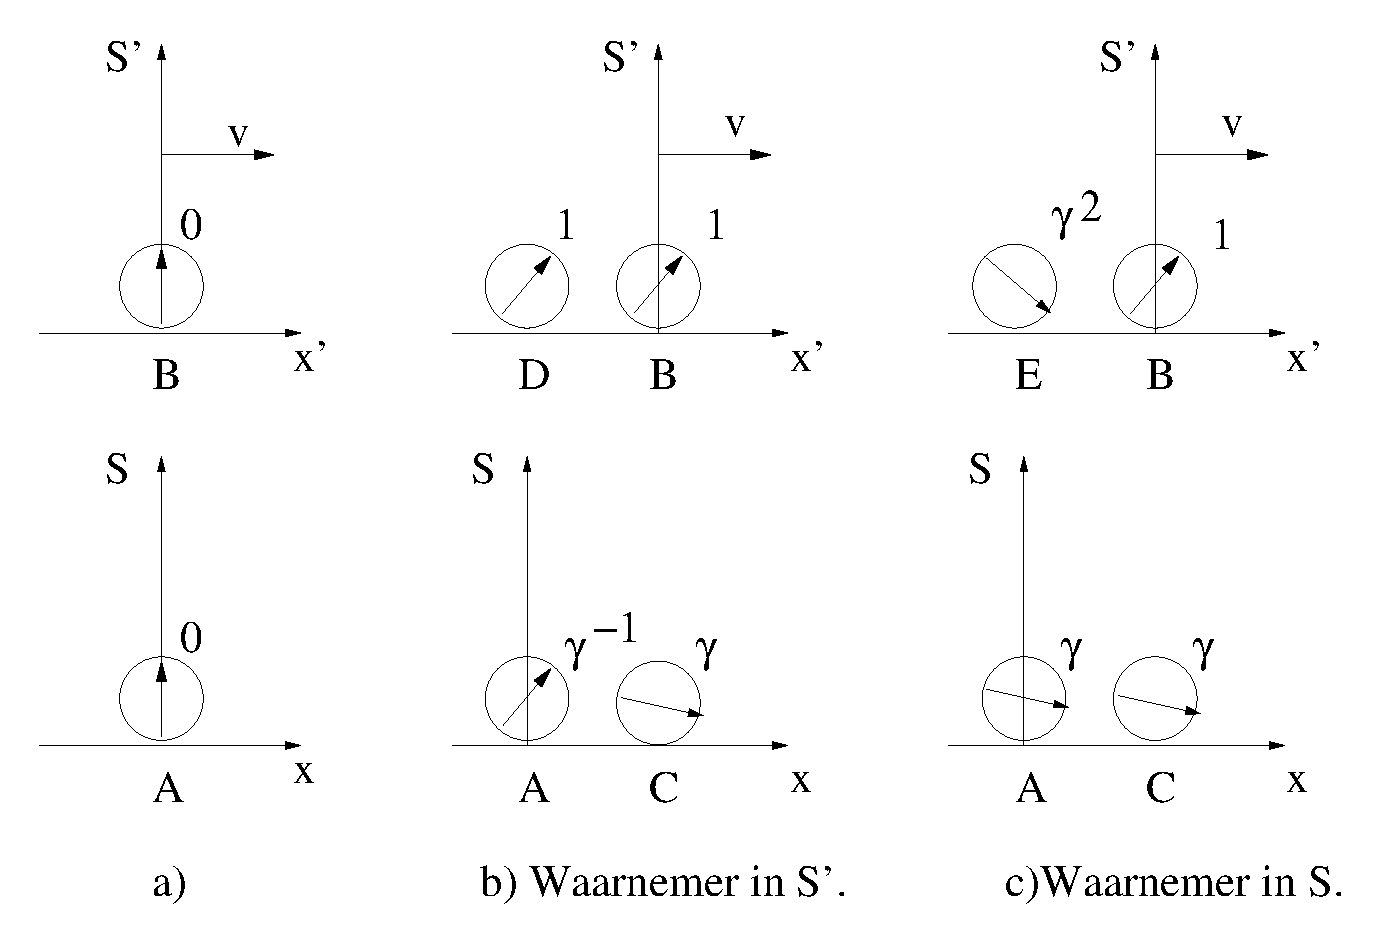
\includegraphics[width=.8\textwidth]{oefeningen.pictures/klokken}
\caption{Klokken}
\label{f:klokken}
\end{figure}

Als klok $B$ klok $A$ passeert staan ze beide op 0: $ct'=0$ en $ct=0$
(zie figuur \ref{f:klokken}a).


Even later, als klok $B$ op $ct'=1$ staat, passeert hij klok $C$ in $S$,
die dan op $ct=\gamma$ staat (zie fig. \ref{f:klokken}b).Volgens een waarnemer in $S'$ staat klok $A$ dan op $ct = \gamma^{-1}$ en 
passeert hij klok $D$ in $S'$, die dan op $ct'=1$ staat 
(fig. \ref{f:klokken}b). Volgens een waarnemer in $S$ staat klok $A$ dan op $ct=\gamma$ en 
passeert klok $A$ klok $E$, die dan $ct'=\gamma^{2}$ aanwijst in $S'$  (zie fig. \ref{f:klokken}c).

\begin{itemize}
\item [a.]
Schrijf de Lorentztransformatie tussen $S$ en $S'$ op.
\item [b.]
Controleer met de Lorentztransformatie de opgegeven stand van de klokken.
\item [c.]
Waar zie je tijddilatatie optreden?

\end{itemize}


%%%%%%%%
\subsection{Raketten 2}\label{prob:rak4}
$S$ is het inertiaalsysteem van de aarde. 
Raket $P$ passeert de aarde op $t$ = 0 met snelheid $\frac{1}{2}c$ en 
beweegt zich naar raket $Q$ die de aarde met $\frac{1}{2}c$ nadert (zie
figuur \ref{f:raket}. 

% \begin{figure}
% \begin{center}
% \mbox{\epsfxsize=8cm\epsffile{oefeningen.pictures/rockets.eps}}
% \caption{Raketten}
% \label{f:raket}
% \end{center}
% \end{figure}

\begin{figure}[ht]
\centering
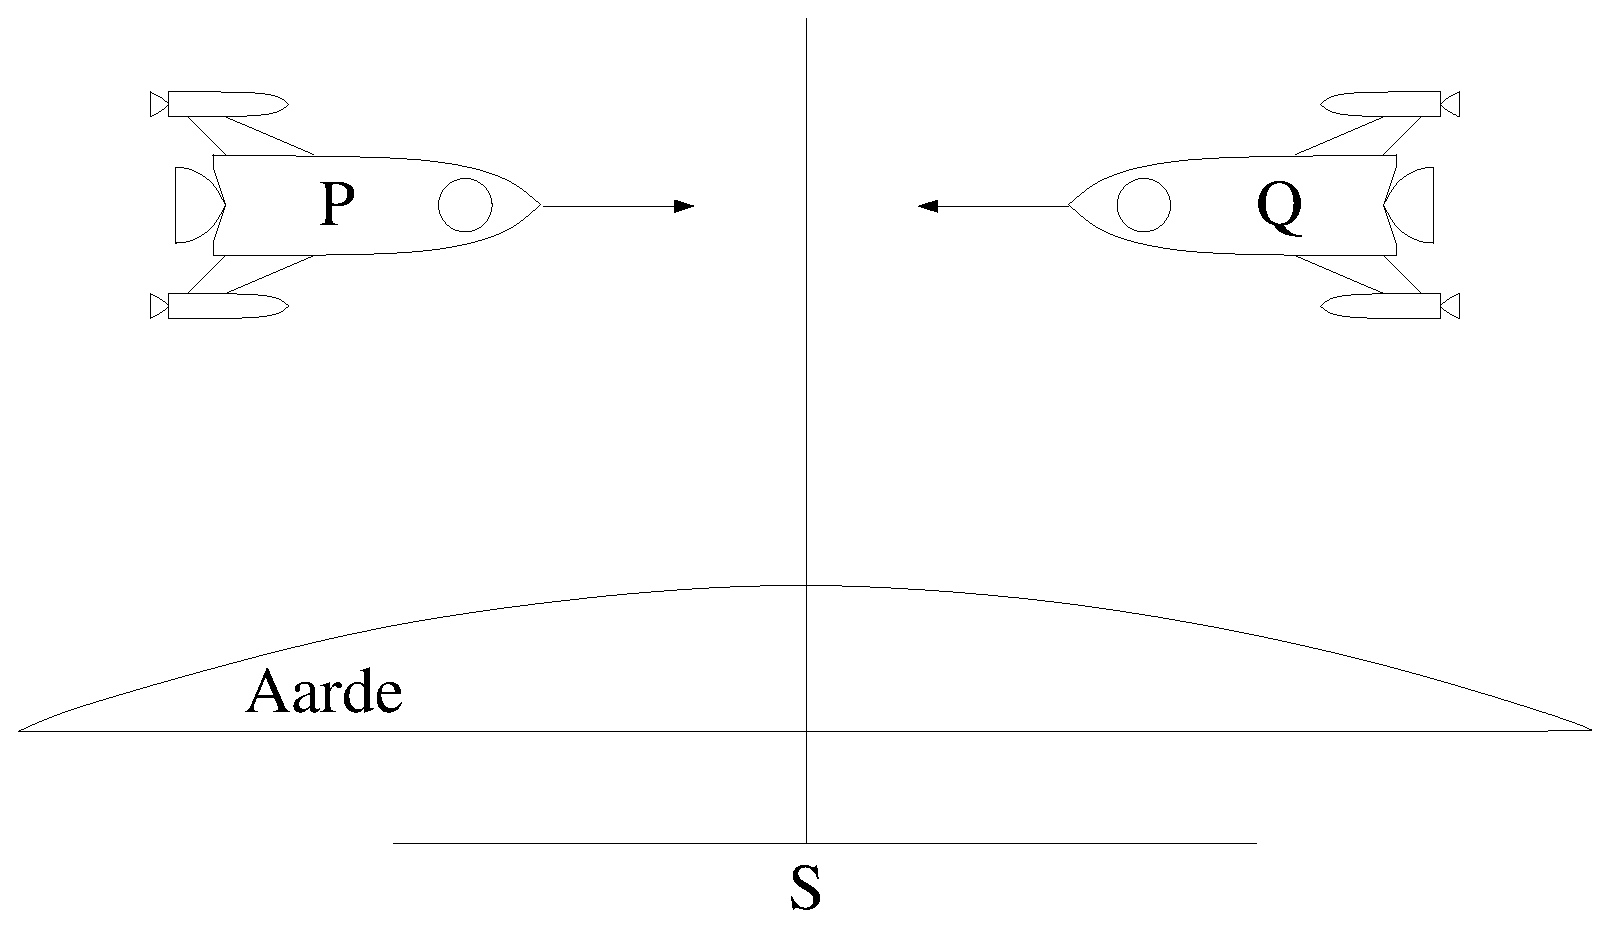
\includegraphics[width=.5\textwidth]{oefeningen.pictures/rockets}
\caption{Raketten}
\label{f:raket}
\end{figure}



Volgens  een waarnemer op aarde bevindt $Q$ zich op $t = 0$ op een afstand
$x = 4$ (lichtjaar), zodat $P$ 
en $Q$ elkaar in $x = 2$ (lichtjaar) zullen ontmoeten, na $t = 4$ jaar 
(dus $ct = 4$ lichtjaar). 
\begin{itemize}
\item [a.]
  Noteer  de  $x$-  en $ct$-co\"{o}rdinaten van de start van $P$,
de start van $Q$ en 
hun ontmoeting.
\end{itemize} 
We bekijken de gebeurtenis nu vanuit raketje $P$ (stelsel $S'$).
\begin{itemize}
\item [b.]
  Schrijf de Lorentztransformatie van $S$ naar $S'$ op (let op + en - tekens!)
\item [c.] 
  Vertaal  de  start  van $P$ en $Q$ en hun ontmoeting naar 
$S'$-co\"{o}rdinaten en noteer hiervan de $x'$- en $ct'$-co\"{o}rdinaten.
\item [d.]
  Welke  snelheid  $v' = \Delta x'/\Delta t'$ had raket $Q$, 
gezien vanuit $P$? 
Controleer dat met de snelheids-optelformule.
\end{itemize} 

%%%%%%%
\subsection{Lichtflitsen}
In een inertiaalsysteem $S$ worden in $A$ en $B$, $5$ $\mu$s na elkaar lichtflitsen uitgezonden.
De afstand $AB$ is $5$ km.
Als je in $S$ met een bepaalde snelheid $v$ parallel aan de lijn $AB$ beweegt, 
zie je de flitsen gelijktijdig.
Hoe groot moet $v$ zijn?


%%%%%%%
\subsection{Trein}
Een trein met een lengte $L_{0}$ (als hij stilstaat) davert langs een station
waarvan het perron een lengte $L < L_{0}$ heeft.
\begin{itemize}
\item [a.]
Hoe groot moet zijn snelheid zijn, zodat volgens iemand op het perron de staart
van de trein aan de achterkant van het perron is op hetzelfde moment als de kop van de trein aan de voorkant is?
\end{itemize}
Twee mensen aan de uiteinden van het perron slaan gelijktijdig 
(volgens hun eigen waarneming) een deuk in de trein.
\begin{itemize}
\item [b.]
Op welke afstand liggen die deuken uit elkaar volgens de mensen op het perron?
\item [c.]
En volgens de mensen in de rijdende trein?
\item [d.]
Waar zitten de deuken als de trein gestopt is?
\end{itemize}

%%%%%%%%%%%
%\subsection{Bewegende lichtklok}
%Ga na dat de lichtklok in figuur 4.2 op blz. 18 van de syllabus `tikt'
%als in formule 4.1 op blz. 17 van de syllabus.

		%bijgewerkt 21:00-16/01/2009
\section{Minkowski-diagrammen}

%afbeeldingen draaien enz.
% 5.6 toevoegen.

%%%%%%%%
\subsection{Drie gebeurtenissen}
Gebeurtenissen worden vanuit drie standpunten bekeken die een onderlinge 
beweging hebben: $S_{1}$, $S_{2}$ en $S_{3}$. 

% \begin{figure} [h]
% \begin{center}
% \mbox{\epsfxsize=10cm\epsffile{oefeningen.pictures/oef_4/oef4-1.eps}}
% \caption{Drie gebeurtenissen}
% \label{f:oef4-1}
% \end{center}
% \end{figure}

\begin{figure}[ht]
\centering
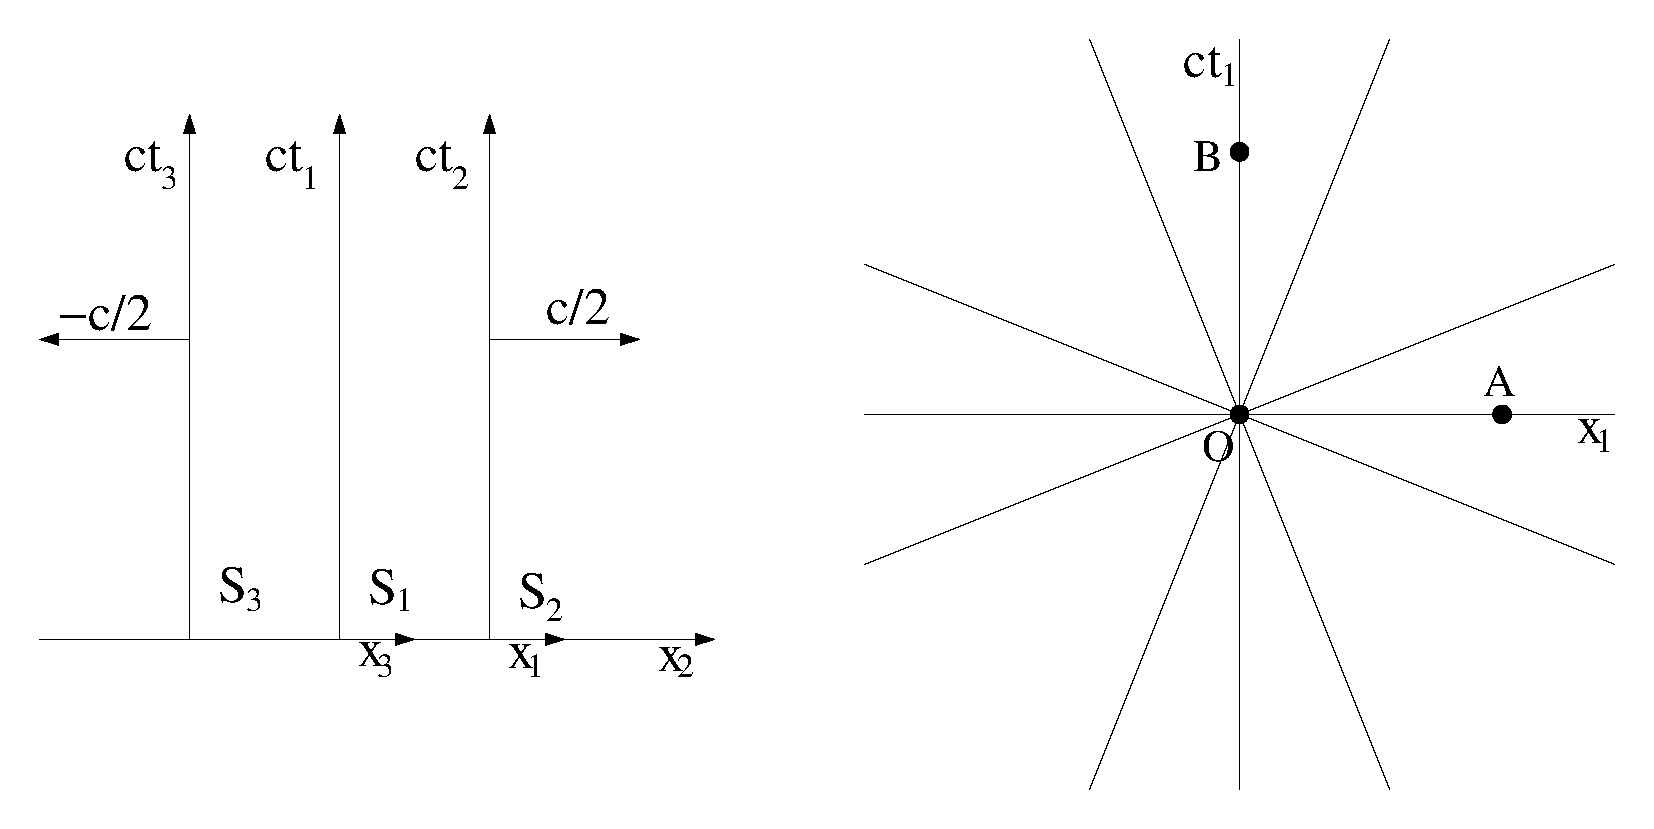
\includegraphics[width=.8\textwidth]{oefeningen.pictures/oef_4/oef4-1}
\caption{Drie gebeurtenissen}
\label{f:oef4-1}
\end{figure}  

In het Minkowski-diagram van $S_{1}$ zijn drie "gebeurtenissen" $O$, $A$ en $B$
aangegeven. 
\begin{itemize}
\item [a.]
  Geef in het rechter diagram aan wat de $x_{2}$-, $ct_{2}$-, $x_{3}$- en
  $ct_{3}$-assen zijn. 
\item  [b.]
  Volgens $S_{1}$ is gebeurtenis $A$ gelijktijdig met gebeurtenis $O$. 
Hoe zit dat in $S_{2}$ en $S_{3}$? 
\item [c.]
  In  $S_{1}$ stelt de overgang van $O$ naar $B$ een toestand van rust voor. 
Hoe zit dat in $S_{2}$ en in $S_{3}$? 
\end{itemize}

%%%%%%%
\subsection{Draaing in het $ct,x$-diagram}
We kijken naar twee stelsels $S$ en $S'$ die verbonden zijn door de 
Lorentztransformatie (zie figuur \ref{f:rotate}):
\begin{eqnarray*}
   x & = & \gamma (x' + \beta ct')  \\
  ct & = & \gamma(ct'+\beta x')
\end{eqnarray*}  

% \begin{figure} [h]
% \begin{center}
% \mbox{\epsfxsize=10cm\epsffile{oefeningen.pictures/oef_4/rotate.eps}}
% \caption{Draaiing van assen}
% \label{f:rotate}
% \end{center}
% \end{figure}

\begin{figure}[ht]
\centering
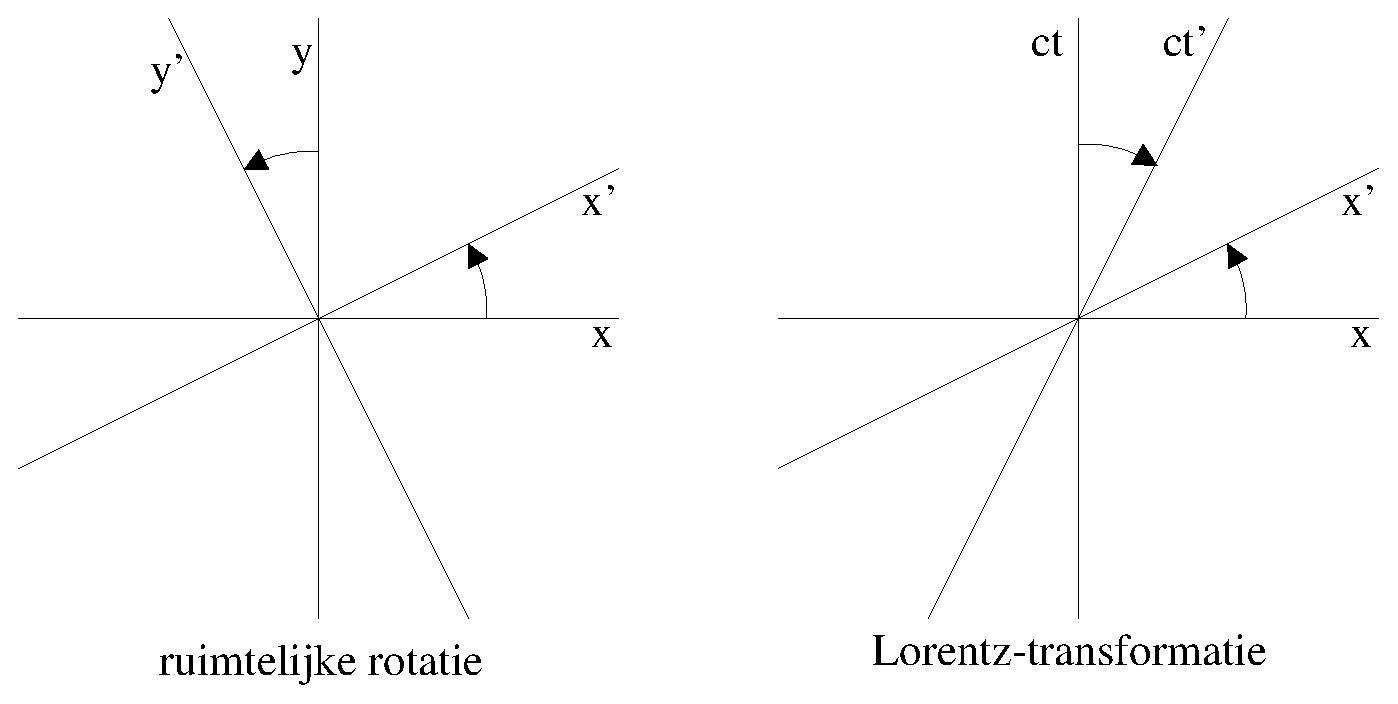
\includegraphics[width=.8\textwidth]{oefeningen.pictures/oef_4/rotate}
\caption{Draaiing van assen}
\label{f:rotate}
\end{figure}

De  Lorentztransformatie  veroorzaakt  een soort draaiing in het 
$ct$,$x$-diagram, die lijkt op een 
gewone  ruimtelijke  rotatie in het $x,y$-vlak, met het verschil dat 
de $ct$- en $x$-assen beide naar 
binnen draaien, over een hoek $\alpha$ met $\tan{\alpha} = \beta = v/c$ :

\begin{itemize}
\item [a.]
  Laat  zien  dat  de  $x'$-as  (de  lijn  met  $ct' = 0$)  in  het  
$ct$,$x$-diagram  een lijn met 
  richtingsco\"{e}ffici\"{e}nt $\beta$ is (dus van de vorm $ct = \beta x$ is).
\item [b.]
  Laat ook zien dat de $ct'$-as (dus de lijn met $x' = 0$) een
  richtingsco\"{e}ffici\"{e}nt $\beta$ heeft met de 
  $ct$-as (dus van de vorm $x = \beta ct$ is).
\end{itemize}

Terwijl  bij  een  rotatie  in  het  $x,y$-vlak  de  eenheden  op de 
gedraaide assen liggen op de eenheidscirkel  $x^{2} + y^{2} = 1$,  
zo liggen de eenheden van de gekantelde $ct'$,$x'$-assen op de eenheids 
hyperbolen $x^{2} - (ct)^{2}= \pm 1$ (figuur \ref{f:eenheid}):

% \begin{figure} [h]
% \begin{center}
% \mbox{\epsfxsize=10cm\epsffile{oefeningen.pictures/oef_4/eenheid.eps}}
% \caption{Eenheden}
% \label{f:eenheid}
% \end{center}
% \end{figure}

\begin{figure}[ht]
\centering
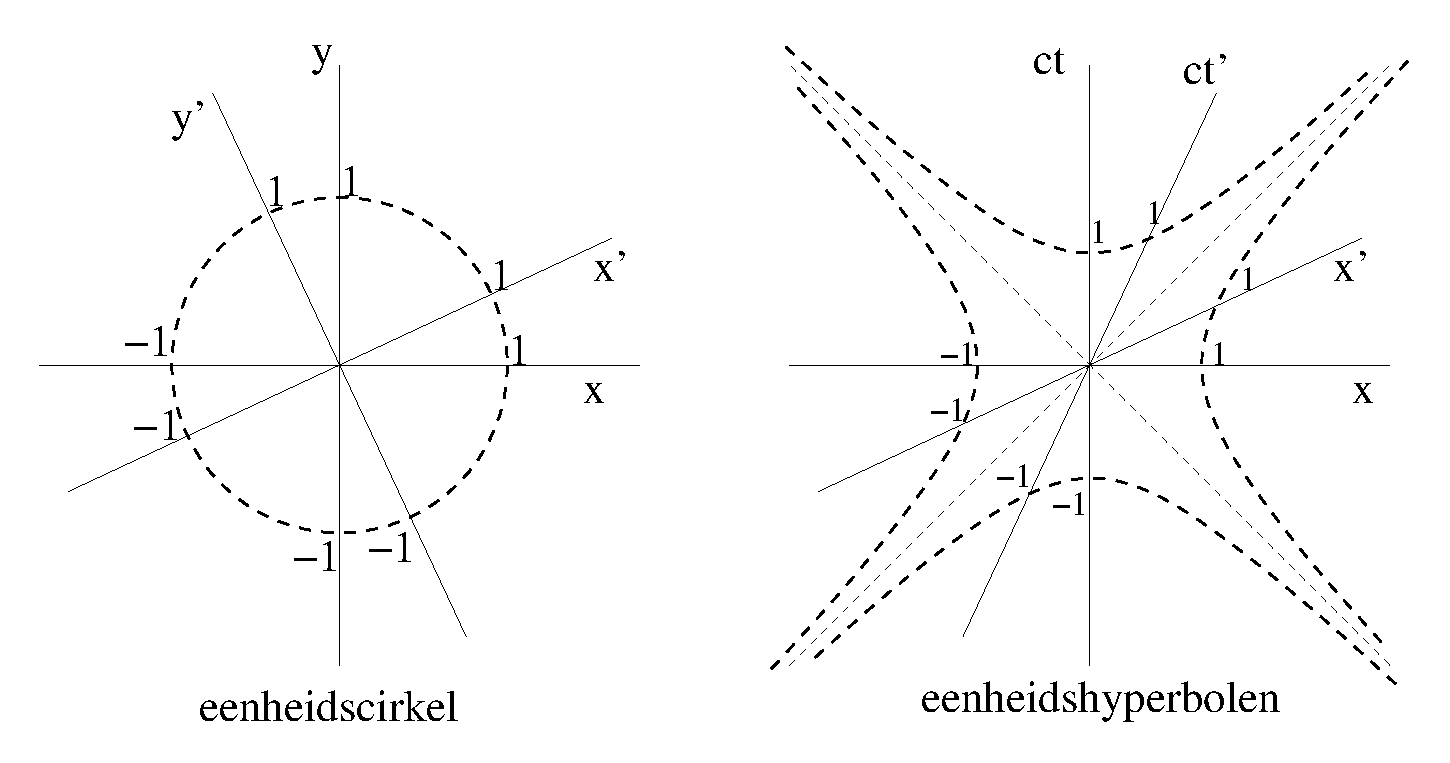
\includegraphics[width=.8\textwidth]{oefeningen.pictures/oef_4/eenheid}
\caption{Eenheden}
\label{f:eenheid}
\end{figure}

%eenheids-                                      eenheids-
% cirkel                                       hyperbolen
%$x_{1}^{2}+y_{1}^{2}=1$                    $x_{1}^{2}-(ct_{1})^{2}=\pm 1$

\begin{itemize}
\item [c.]
  Reken  voor  de  eenheden  op de $x'$-as (dus $ct' = 0$ en
  $x' = \pm 1$) na dat de bijbehorende $x$- en 
  $ct$-getallen voldoen aan $x^{2} - (ct)^{2} = +1$.
\item [d.]
  Hetzelfde voor de eenheden op de $ct'$-as: $x^{2} - (ct)^{2} = -1$.
\end{itemize}


%%%%%%%%%%
\subsection{Lorentzcontractie en Tijddilatatie in Minkowski-diagram}


%\begin{figure}[ht]
%\centering
%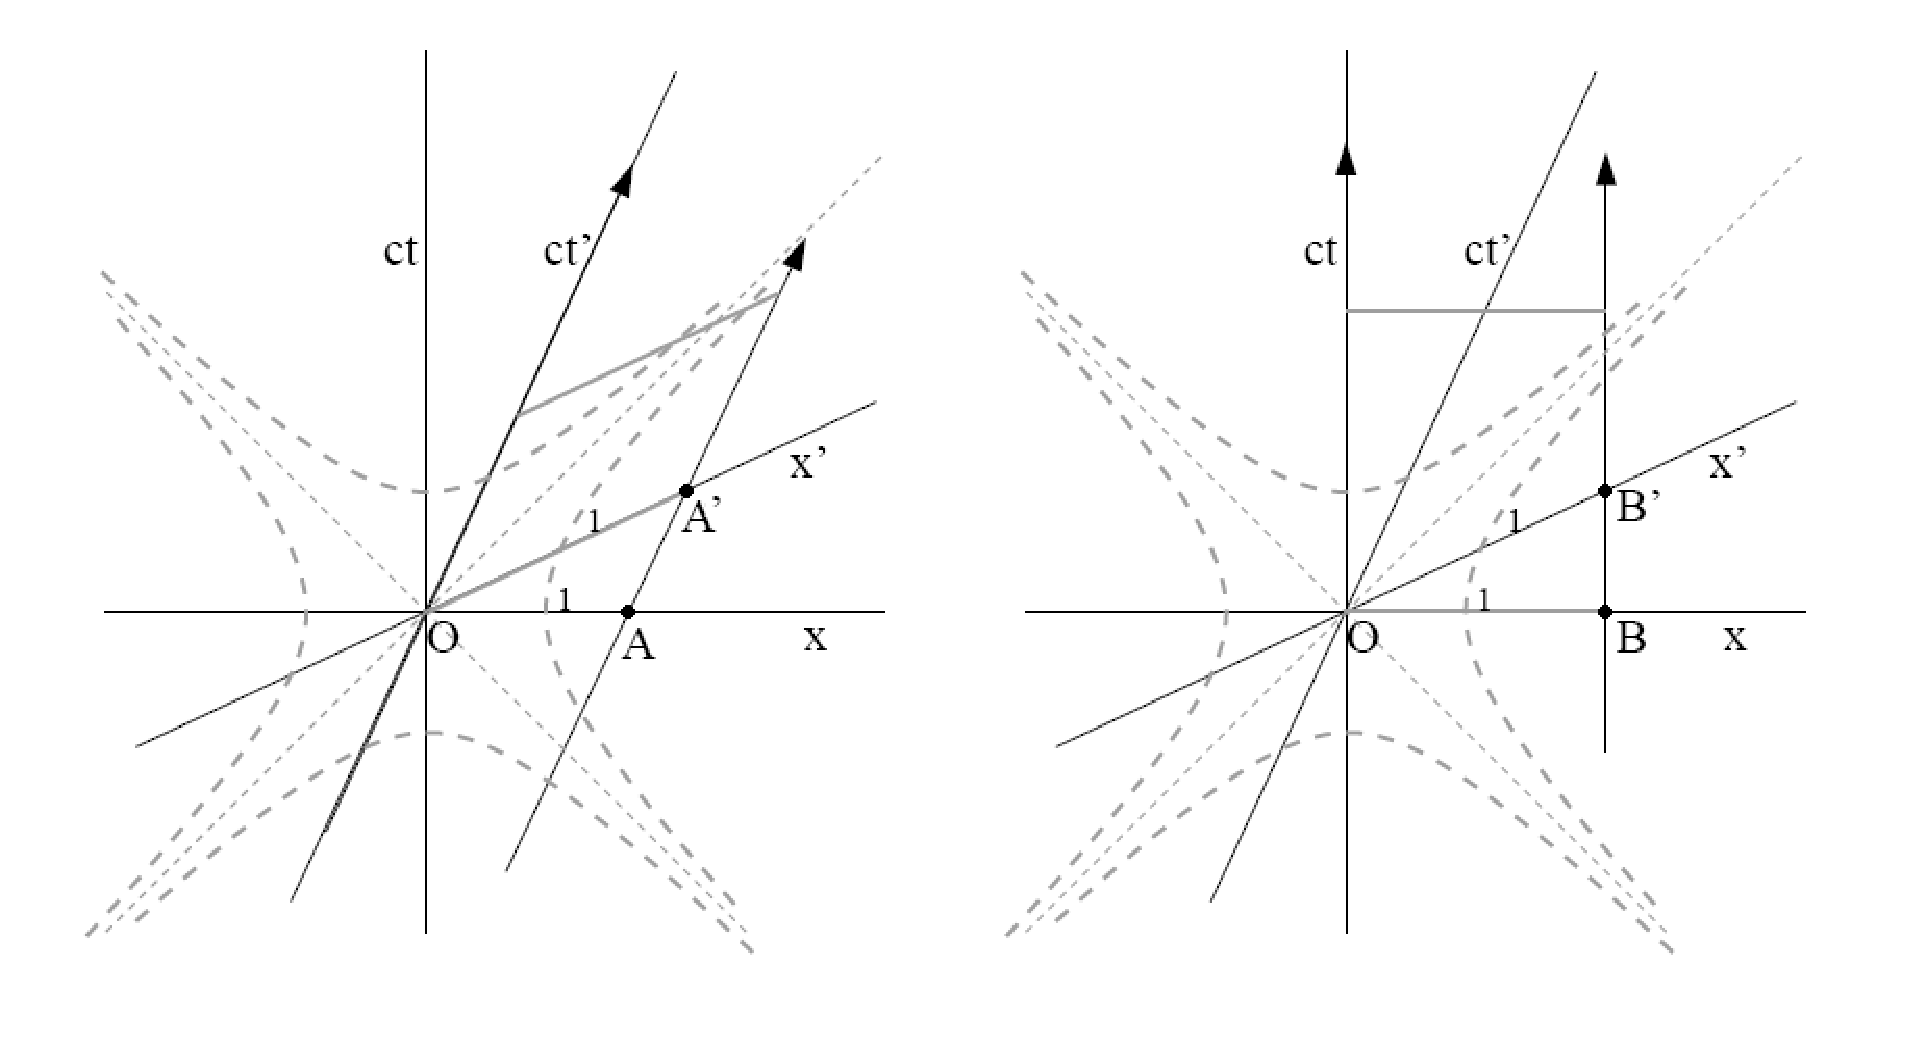
\includegraphics[width=0.8\textwidth]{contractiediag1}
%\caption{Lorentzcontractie}
%\label{f:mcontractie}
%\end{figure}

\begin{figure}[ht]
 \begin{center}
 \mbox{\epsfxsize=10cm\epsffile{oefeningen.pictures/contractiediag1.eps}}
 \caption{Tijddilatatie}
 \label{f:mcontractie}
 \end{center}
 \end{figure}


 Lorentzcontractie met een Minkowski-diagram: 
\begin{itemize}
\item [a.]
 Toon  met  de  twee diagrammen van figuur \ref{f:mcontractie} aan dat een 
lat $OA'$
 (met lengte 2) in $S'$, gezien vanuit $S$ verkort 
 is, en andersom, dat een lat $OB$ in $S$, verkort is in $S'$.
\end{itemize}

%\begin{figure}[h]
%	\centering
%		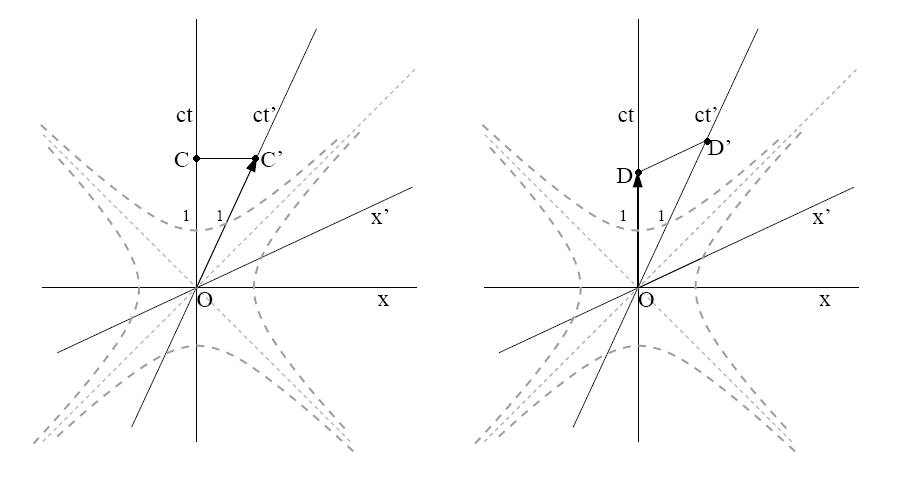
\includegraphics[width=0.8\textwidth]{contractiediag2.EPS}
%	\caption{Tijddilatatie}
%	\label{f:mtijddil}
%\end{figure}

 \begin{figure}[ht]
 \begin{center}
 \mbox{\epsfxsize=10cm\epsffile{oefeningen.pictures/contractiediag2.eps}}
 \caption{Tijddilatatie}
 \label{f:mtijddil}
 \end{center}
 \end{figure}

  Tijddilatatie in een Minkowski-diagram:
\begin{itemize}
\item [b.]
Laat in de diagrammen van figuur \ref{f:mtijddil} zien dat een klok, 
die in $S'$ van $O$ naar $C'$ loopt, vanuit $S$ gezien langzamer is, 
en andersom, dat een klok die in $S$ van $O$ naar $D$ loopt, vanuit $S'$ gezien 
langzamer is.
\end{itemize}


%%%%%%%%%%%
\subsection{Wereldlijnen}
In  het  co\"{o}rdinatenstelsel $S$ staan $A$ en $B$ stil op de plaatsen
$x_{A} = 0$ en $x_{B} = 3$. 
Op $t = 0$ zendt $A$ 
een lichtgolf uit die $B$ bereikt op $t = \frac{3}{c}$. 

% \begin{figure} [h]
% \begin{center}
% \mbox{\epsfxsize=10cm\epsffile{oefeningen.pictures/oef_4/kleurplaat.eps}}
% \caption{Teken wereldlijnen}
% \label{f:kleurplaat}
% \end{center}
% \end{figure}


\begin{figure}[ht]
\centering
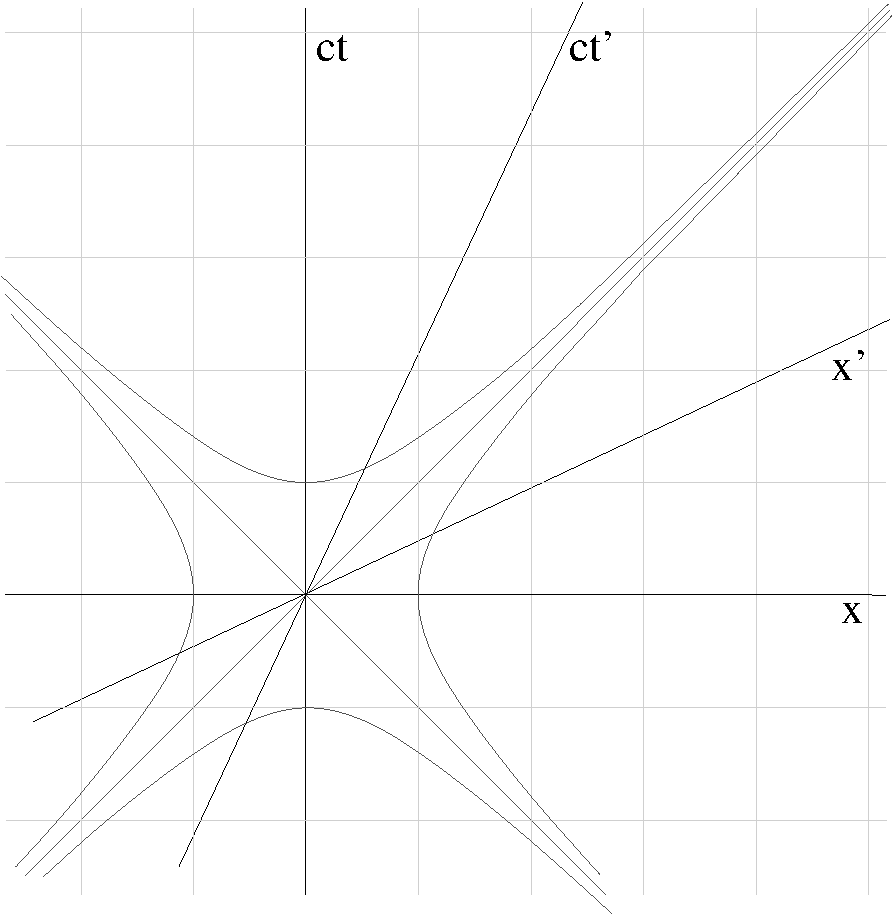
\includegraphics[width=.8\textwidth]{oefeningen.pictures/oef_4/kleurplaat}
\caption{Teken wereldlijnen}
\label{f:kleurplaat}
\end{figure}

\begin{itemize}
\item [a.]
  Teken in het Minkowski-diagram in figuur \ref{f:kleurplaat}
  de zgn. wereldlijnen van $A$ en $B$ 
(dus de lijnen $x = 0$ 
  en $x = 3$). Teken ook het punt $C$: de gebeurtenis waar het licht vanuit $A$, $B$ bereikt. 
\end{itemize}
Een  ander stelsel $S'$ beweegt met $\frac{1}{2}c$ t.o.v. $S$ in de positieve 
$x$-richting.
De $x'$,$ct'$-assen zijn 
al in het diagram aangegeven. 

\begin{itemize}
\item [b.]
  Controleer dat de snelheid van $S'$ t.o.v. $S$ gelijk is aan $\frac{1}{2}c$ 
  en geef 
het punt $B'$ aan waar 
  $B$ zich volgens $S'$ bevindt op het ogenblik dat het licht uit $A$ 
vertrekt. 
\item [c.]
  Bereken  de  $ct'$,$x'$  co\"{o}rdinaten  voor  de  punten  $B'$  en  $C$ 
(gebruik daarbij de Lorentztransformatie) 
\item [d.]
  Bereken uit de $x'$- en $t'$-verschillen tussen $B'$ en $C$ hoe snel $B$ 
beweegt in $S'$; bereken uit 
  de  $x'$-  en  $ct'$-verschillen  tussen de oorsprong $O$ en $C$ hoe groot 
de lichtsnelheid in $S'$ is. 
  Waren deze antwoorden te verwachten? 
\end{itemize}

%%%%%%%%%%%%%
\subsection{Opnieuw raketten}
Nog een keer de situatie van de opgave `Raketten 2' (opgave \ref{prob:rak4}).

% \begin{figure} [h]
% \begin{center}
% \mbox{\epsfxsize=10cm\epsffile{oefeningen.pictures/oef_4/kleurplaat.eps}}
% \caption{Teken raketbewegingen}
% \label{f:kleurplaat2}
% \end{center}
% \end{figure}

\begin{figure}[ht]
\centering
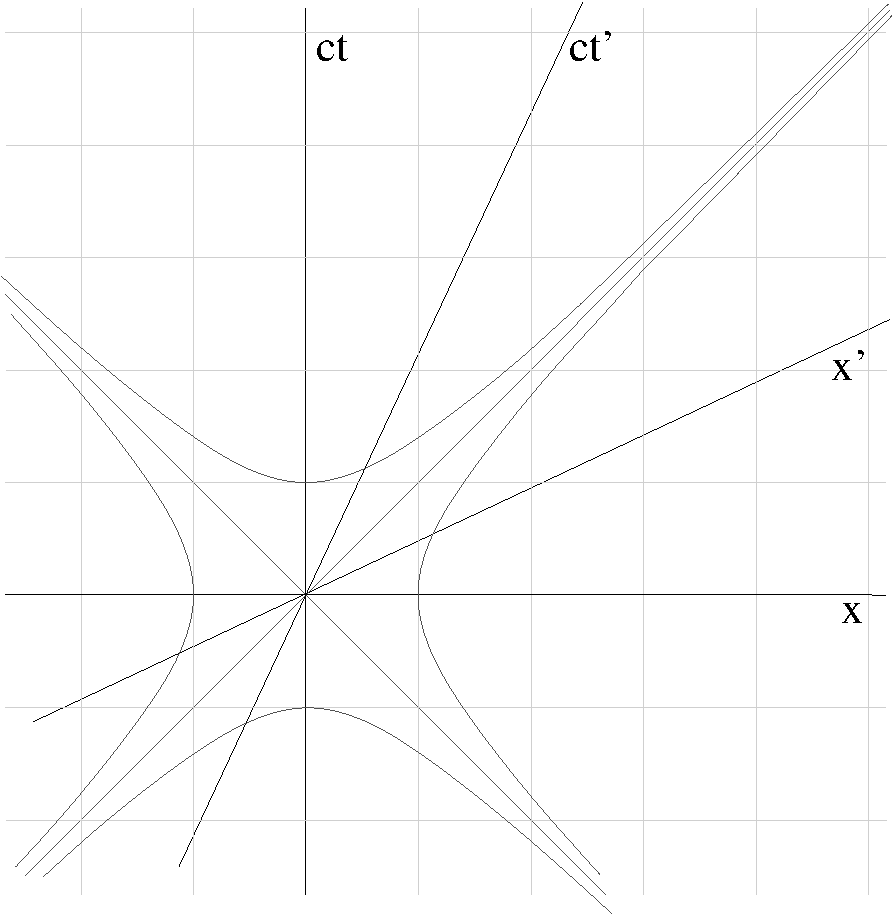
\includegraphics[width=.8\textwidth]{oefeningen.pictures/oef_4/kleurplaat}
\caption{Teken raketbewegingen}
\label{f:kleurplaat2}
\end{figure}

\begin{itemize}
\item [a.]
Teken de beweging van $P$ en $Q$ in het Minkowski-diagram in figuur \ref{f:kleurplaat2}. 
 
\item [b.]
  Teken de $x'$,$ct'$ assen die gelden voor een waarnemer ($S'$) die met 
raket $P$ mee beweegt. 
\item [c.]
  Hoe groot is volgens $S'$ op $t' = 0$ de afstand $x'$ tot raket $Q$? 
(uit het diagram aflezen) 
\item [d.]
  Na hoeveel tijd ontmoeten $P$ en $Q$ elkaar in $S'$? (uit het diagram
  aflezen).
\item [e.]
Bereken  de  snelheid  van  $Q$  in  $S'$  uit  de $x'$-verplaatsing van $Q$
tussen $ct' = 0$ en zijn ontmoeting met $P$. 
Vergelijk het antwoord met vraag d) van de opgave `Raketten' uit hoofdstuk \ref{CLT}.
\end{itemize}

%\newpage
%Gebruik voor het huiswerk onderstaande figuur.
%
%% \begin{figure} [h]
%% \begin{center}
%% \mbox{\epsfxsize=10cm\epsffile{oefeningen.pictures/oef_4/kleurplaat.eps}}
%% \caption{Teken raketbewegingen}
%% \end{center}
%% \end{figure}
%
%\begin{figure}[ht]
%\centering
%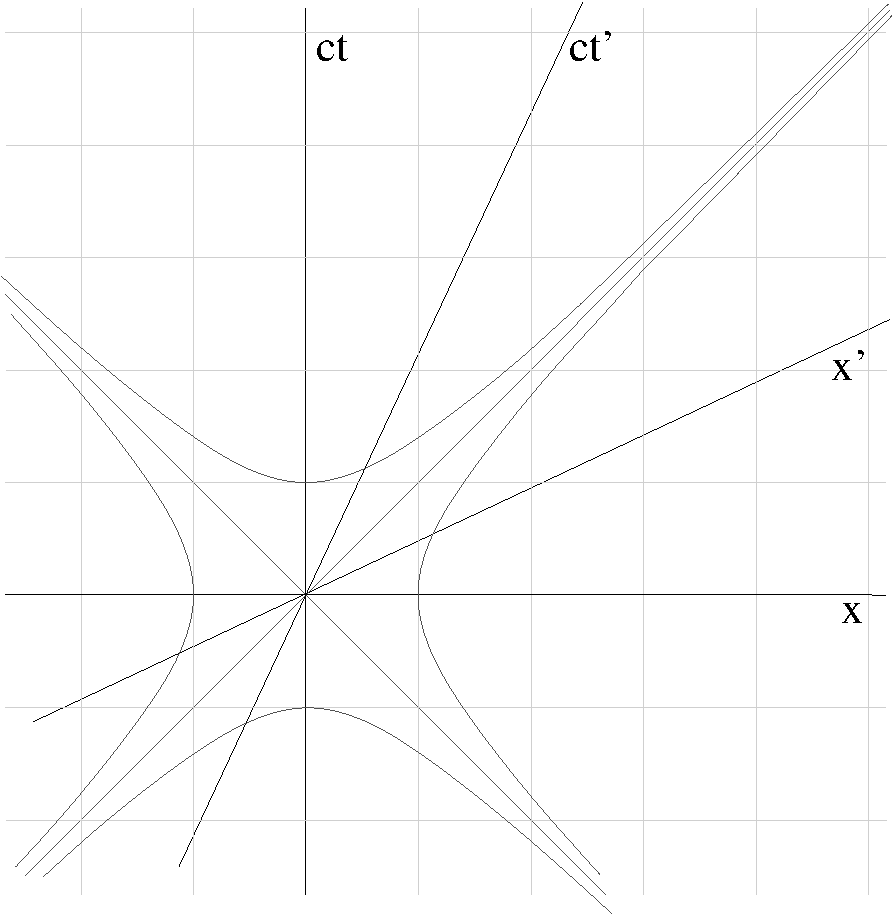
\includegraphics[width=1.0\textwidth]{oefeningen.pictures/oef_4/kleurplaat}
%\caption{Teken raketbewegingen}
%\end{figure}

%%%%%%%%%
\subsection{Nogmaals raketten}

			Hieronder zie je twee onvolledige Minkowski-diagrammen, die horen bij de eerder gemaakte opdracht \ref{prob:rak3}. Het ene diagram
toont de situatie zoals waargenomen vanuit $S$, de andere zoals waargenomen
vanuit $S'$. Geef in beide diagrammen aan of de assen $ct'$ of $x'$, danwel $ct$ of $x$ zijn. Geef verder in
ieder van de diagrammen aan wat de wereldlijnen zijn van $P$ en $Q$. Teken ten
 slotte in ieder van de diagrammen een lichtstraal die uitgezonden wordt
door $P$ in de richting van $Q$ (de aankomst van de lichtstraal bij $Q$ zou
buiten de tekening kunnen vallen).
			
			

 \begin{figure} [h]
 \begin{center}
 \mbox{\epsfxsize=14cm\epsffile{oefeningen.pictures/MinkS.eps}}
 \caption{Onvoltooid Minkowski diagram in stelsel S}
 \label{f:MinkS}
 \end{center}
 \end{figure}
 
  \begin{figure} [h]
 \begin{center}
 \mbox{\epsfxsize=14cm\epsffile{oefeningen.pictures/Minkowski_Saccent.eps}}
 \caption{Onvoltooid Minkowski diagram in stelsel S'}
 \label{f:MinkSac}
 \end{center}
 \end{figure}

%\begin{figure}[h]
%	\centering
%		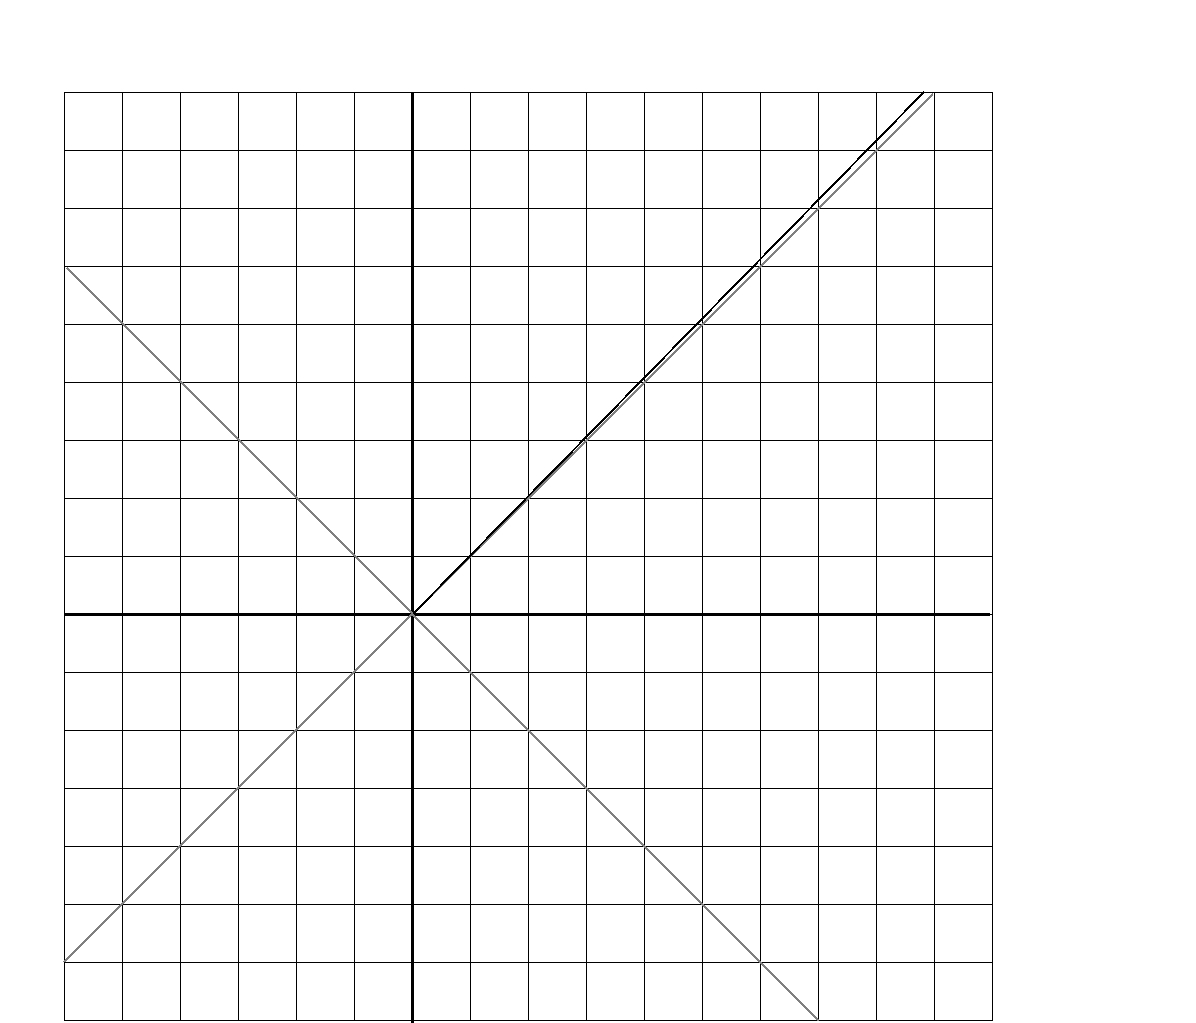
\includegraphics[width=0.68\textwidth]{Minkowski_Saccent.png}
%	\caption{Bijlagen bij vraag 3h).}
%	\label{fig:raketten}
%\end{figure}
%
%\begin{figure}[h]
%	\centering
%		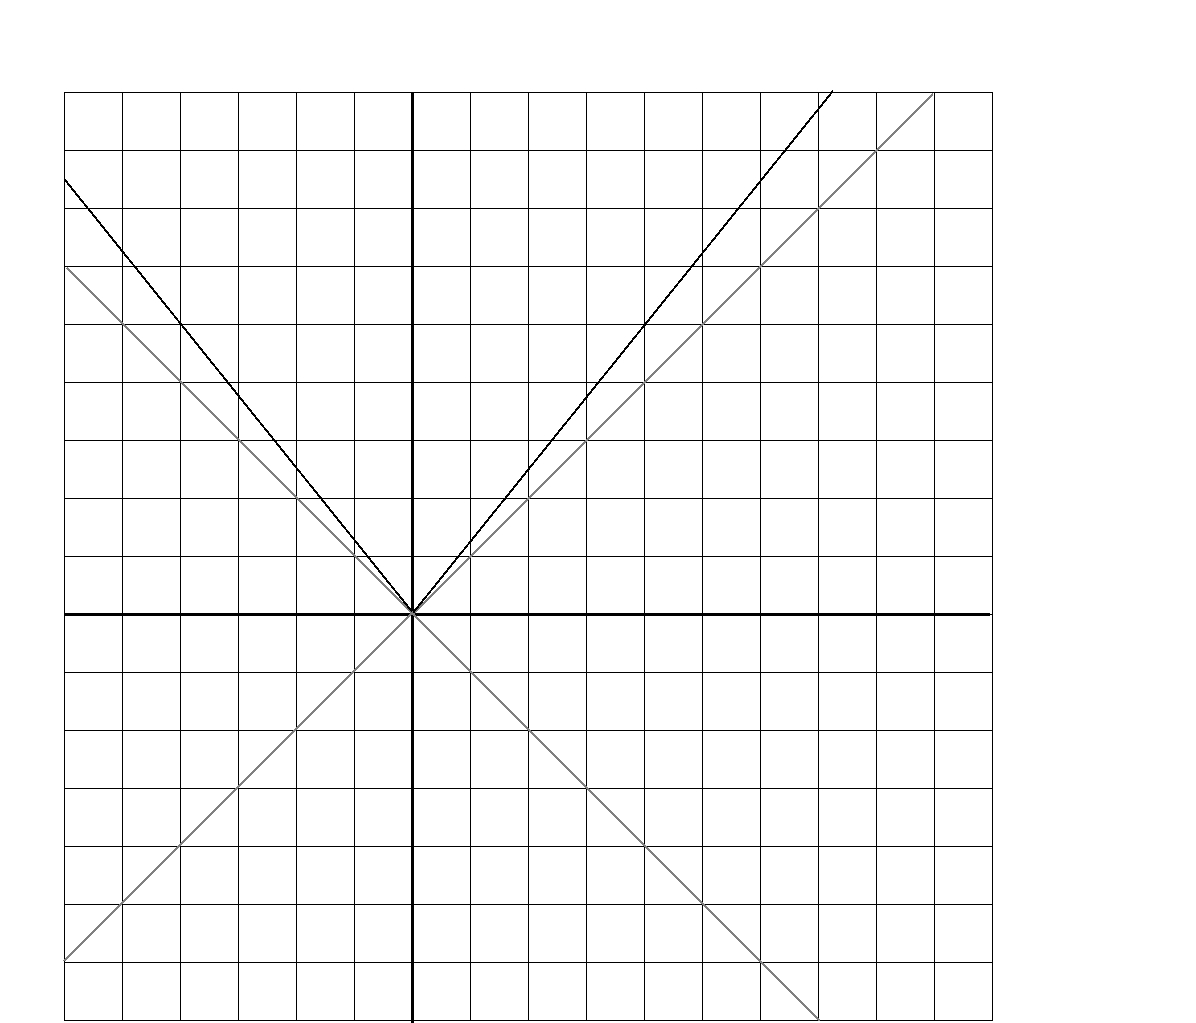
\includegraphics[width=0.68\textwidth]{Minkowski_S.png}
%	\caption{Bijlagen bij vraag 3h).}
%	\label{fig:raketten2}
%\end{figure}


%%%%%%%%%%%%
%\subsection{}
%In  het  Minkowski diagram in figuur \ref{} zijn de co\"{o}rdinaat-assen voor twee 
%inertiaalstelsels $S$ en 
%$S'$  getekend  die  een  onderlinge  snelheid langs de $x$-as hebben. 
%Voor de tijdseenheden kunnen 
%jaren worden gelezen, voor de lengte eenheden lichtjaren. 
%\begin{itemize}
%\item [a.]
%  Ga na dat die snelheid gelijk is aan $c/5$.
%\item [b.] 
%  Geef  met  een lijnstuk $OP$ geeft de reis aan van iemand ($B$) die twee 
%jaar met $S'$ mee beweegt. 
%  In $S$ blijft iemand anders ($A$) achter. 
%  Hoeveel tijd is er volgens A verlopen ($ct_{1}$) als de klok van B op c$t_{2}$=2 (jaar) staat? Loopt 
%  de tijd in $S_{2}$ volgens A te snel of te langzaam? 
%\end{itemize}
%  c)  Welk  tijdstip ($ct_{1}$) wijst de klok van A volgens B aan, als de klok van B op c$t_{2}$=2 staat? 
%  Loopt de tijd in $S_{1}$ volgens B te snel of te langzaam? 
%In  P  keert  B  om en beweegt met een even grote snelheid (-5c) terug naar A. Hij bereikt A in 
%punt Q. 
%  d) Teken de x3,ct3 assen door de oorsprong die voor het stelsel $S_{3}$ gelden waarin B zich op de 
%  terugreis bevindt. 
%  e)  Zodra  B  in  punt  P  aan  de  terugreis  begint  (en dus plotseling in stelsel $S_{3}$ zit), 
%  verspringt volgens hem de klok van A. Welke $ct_{1}$ ziet B dan? 
%  f) Hoeveel tijd duren de heen- en terugreis volgens B zelf? 
%  g) Hoeveel tijd is er volgens A voor de hele reis nodig geweest? 
%  In  de  vragen  b)  en c) was het zo dat A en B van elkaar vonden dat de klok van de ander te 
%  langzaam  ging.  Nu ze weer bij elkaar zijn, blijkt dat er voor B minder tijd is verlopen dan 
%  voor A (dit is de tweelingparadox). 
%  h) Waarom heeft B er geen recht op om te zeggen dat de tijd in A te langzaam liep? 
				%bijgewerkt 15:15-17/01/2009  + extra  
\section{Klassieke Mechanica}
Voor de Klassieke Mechanica zullen een aantal opgaven uit het boek
`Analytical Mechanics' van Fowles \& Cassiday worden behandeld. Dit zijn onder meer:
\begin{itemize}
\item{Hoofstuk 1}: 1.1, 1.2, 1.3, 1.5, 1.6, 1.7
\item{Hoofdstuk 2}: 2.1, 2.2, 2.3, 2.4, 2.6
\item{Hoofdstuk 4}: 4.1, 4.2, 4.3, 4.4, 4.5
\item{Hoofdstuk 7}: 7.1, 7.2, 7.4, 7.5
\end{itemize}
Hieronder volgen een aantal extra opgaven.

%%%%%%%%%%%%
\subsection{Botsende deeltjes}
Voor twee botsende deeltjes $A$ en $B$ bestaat de `wet van behoud van impuls':
\begin{displaymath}
   m_{A}v_{1A} + m_{B}v_{1B} = m_{A}v_{2A} + m_{B}v_{2B}
\end{displaymath}
waar $v_{1A}$ en $v_{1B}$ de snelheden van $A$ en $B$ voor de botsing 
en $v_{2A}$ en $v_{2B}$ de snelheden na de botsing zijn.
$S$ en $S'$ zijn twee \textit{niet relativistische} inertiaalsystemen met een onderlinge snelheid $v$.
Bewijs dat wanneer de behoudswet geldt in $S$, deze ook geldt in $S'$.

%%%%%%%%%%%%
\subsection{Massa-middelpunt}
Het  massa-middelpunt van twee deeltjes is een denkbeeldig punt tussen de 
deeltjes in, waarvan de  plaats,  snelheid  en  versnelling  het  gemiddelde 
is van die van de twee deeltjes, als je tenminste  de  grootste  massa  het  
sterkst  meetelt (gewogen gemiddelde).  
Als de massa's van de deeltjes $m_{1}$ en $m_{2}$ zijn, is hun totale
massa $M =  m_{1} + m_{2}$ en geldt voor hun massa-middelpunt:

\begin{eqnarray*}
   x_{M} & = &  \frac{m_{1}}{M}x_{1} + \frac{m_{2}}{M}x_{2} \\
   v_{M} & = &  \frac{m_{1}}{M}v_{1} + \frac{m_{2}}{M}v_{2} \\
   a_{M} & = &  \frac{m_{1}}{M}a_{1} + \frac{m_{2}}{M}a_{2} 
\end{eqnarray*}

Bij  twee  botsende  deeltjes,  waarop verder geen krachten werken, beweegt 
het massa-middelpunt altijd eenparig.
Je  kunt  dan altijd een Galileitransformatie maken van het 
$L$-systeem (het `laboratorium-systeem') waarin de botsing plaats heeft, 
naar het 
$M$-systeem (het `massamiddelpunt-system')\footnote{In het Engels heet dit het `Centre of mass system', ofwel CM-system.}.

Deeltje $A$ heeft een massa $m_{A} = 4$ kg en botst met een snelheid
$v_{A} = 10 $ m/s op een stilstaand 
deeltje $B$  met massa $m_{B} = 1 $ kg. 
\begin{itemize}
\item [a.]
Laat zien dat de totale impuls in het $M$-systeem
v\'{o}\'{o}r  de  botsing nul is:
$p_{A,M} + p_{B,M} = 0$. 
\end{itemize}

In het $M$-systeem zijn (en blijven) de twee impulsen dus {\it even groot} en 
{\it tegengesteld} aan elkaar!

Bij  een  volkomen  elastische  botsing  gaat  er  geen kinetische energie 
verloren.
Het is dan gemakkelijk  te  bewijzen  dat  in het $M$-systeem de impulsen van 
$A$ en $B$ na de botsing niet alleen even groot en tegengesteld zijn, maar 
ook dezelfde grootte hebben als v\'{o}\'{o}r de botsing.
\begin{itemize}
\item [b.]
Als deeltje $A$ bij een volkomen elastische botsing in het $M$-systeem 
$90^{o}$ zou afbuigen, wat zijn dan de snelheden na de botsing 
in het $M$-systeem? 
\item[c.] En in het $L$-systeem? 
\end{itemize}

%%%%%%%%%%%%%
%\subsection{Krachtveld}
% \begin{figure} [h]
% \begin{center}
% \mbox{\epsfxsize=8cm\epsffile{oefeningen.pictures/Krachten.ps}}
% \caption{Krachtveld}
% \label{f:kracht}
% \end{center}
% \end{figure}
%In het $(x,y)$-vlak is de potentiaalfunctie $V(x,y)=x^4y^2$ gedefinieerd. In de figuur zie je een paar lijnen van constante $V$: op de kromme lijnen is $V=1$ en op de $x$- en $y$-as is $V=0$.
%\begin{itemize}
%\item[a.] 
%Bepaal de krachtcomponenten $F_x$ en $F_y$ voor een willekeurig punt $(x,y)$.
%\item[b.]
%Teken de $\vec{F}$-pijl in punt $B$.
%\item[c.]
%Bepaal van dit krachtveld de rotatie: $\mbox{rot} ~\vec{F} \equiv \nabla \times \vec{F}$.
%\end{itemize}



 					%bijgewerkt 13:28-17/01/2009  - krachtveld

%%%%%%%%
%pretest\subsection{electronvolt}
%pretest\begin{itemize}
%pretest\item [a.]
%pretestWat is de definitie van electronvolt?
%pretest\item [b.]
%pretestHoeveel Joule is 1 GeV?
%pretest\item [c.]
%pretestGeef de formule voor de energie van een relativistich deeltje.
%pretest\item [d.]
%pretestDe massa van een electron is $m_{e} = 0,511$ MeV/c$^{2}$.
%pretestWat is de snelheid van een elektron dat een energie van 1 GeV heeft?
%pretest\end{itemize}

%%%%%%%%%%%
%\subsection{Massieve deeltjes}
%Niet-relativistisch heeft een vrij deeltje met massa $m$ en 
%snelheid $v$ een energie $E = \frac{1}{2}mv^{2} = \frac{p^{2}}{2m}$.
%\begin{itemize}
%\item [a.]
%Wat is $\frac{dE}{dp}$?
%\end{itemize}
%Een relativistisch deeltje met massa $m$ en snelheid $v$ heeft een energie
%$E = \sqrt{m^{2}c^{4} + c^{2}p^{2}}$.
%\begin{itemize}
%\item [b.]
%Wat is nu $\frac{dE}{dp}$?
%\item [c.]
%Laat zien waarom het deeltje niet sneller kan bewegen dan de lichtsnelheid.
%\end{itemize}
 

\section{Lorentztransformatie van impuls en energie}

%%%%%%%%
\subsection{Impuls-energie viervector}\label{Ievv}
De componenten van de impulsvector en de energie vormen een vier-vector
$(\frac{E}{c}, p_{x}, p_{y}, p_{z})$ op dezelfde manier als de 
tijd-ruimte-co\"{o}rdinaten $(ct, x, y, z)$.
Bij overgang van stelsel $S$ naar $S'$ transformeren ze volgens dezelfde 
Lorentztransformatie als voor $(x, y, z, ct)$ geldt.
\begin{itemize}
\item [a.]
Vertaal de transformatie 
$x' = \gamma (x - \beta ct),\ ct' = \gamma (ct - \beta x)$ naar
$p_{x}$ en $\frac{E}{c}$.
\end{itemize}
%Als een deeltje stil ligt in $S'$, beweegt het met snelheid $v$ in $S$.
We bekijken een deeltje dat door stelsel $S$ beweegt met snelheid $v$; dit deeltje ligt dus stil in zijn eigen `rustframe' $S'$.
\begin{itemize}
\item [b.]
Laat zien dat je met de Lorentztransformatie voor de impuls en energie van het
bewegende deeltje in $S$ de volgende formules krijgt:
\begin{eqnarray*}
p_{x} &=& \gamma mv\\
E & = & \gamma mc^{2}
\end{eqnarray*}
\end{itemize}
Bij de Lorentztransformatie blijft de combinatie $(ct)^{2} - x^{2}$
hetzelfde, \textit{Lorentzinvariant}.
\begin{itemize}
\item [c.]
Controleer dat voor $(ct)^{2} - x^{2}$ en $(ct')^{2} - x'^{2}$.
\item [d.]
Welke Lorentzinvariante combinatie van $E$ en $p_{x}$ neemt de plaats in van $(ct)^{2} - x^{2}$?
\item [e.]
Welke waarde neemt deze combinatie aan in het rustframe $S'$?
\end{itemize}

%%%%%%%%
\subsection{Energie van een relativistisch deeltje}
Voor een relativistisch deeltje is het verband tussen energie en impuls:
\begin{displaymath}
E^{2} - c^{2}p^{2} = m^{2}c^{4}
\end{displaymath}
dus:
\begin{displaymath}
E = \sqrt{m^{2}c^{4} + c^{2}p^{2}}
\end{displaymath}
\begin{itemize}
\item [a.]
Teken de grafiek van de energie van het bewegende deeltje als functie van 
zijn snelheid $v$.
Geef hierin de bijdrage van de kinetische energie $E_{k} = E - E_{0}$
aan ($E_{0}$ is de rustenergie van het deeltje).
\item [b.]
Hoe snel moet een deeltje bewegen om zijn kinetische energie even groot 
te laten zijn als zijn rustenergie?
\item [c.]
Tot welke uitdrukking reduceert de kinetische energie voor niet-relativistische
deeltjes ($pc \ll E_{0}$)?
\item [d.]
Dezelfde vraag voor relativistische deeltjes ($pc \gg E_{0}$).
\end{itemize}

%%%%%%%
%\subsection{Massa van een relativistisch deeltje}
%Een deeltje met massa $m$ beweegt met snelheid $v = 0,40$c.
%\begin{itemize}
%\item [a.]
%Als je de snelheid van het deeltje verdubbelt, verdubbelt dan ook de impuls 
%van het deeltje zoals je niet-relativistisch zou verwachten?
%Controleer met een berekening.
%\item [b.]
%Als je de impuls van het deeltje verdubbelt, wordt dan de
%kinetische energie van het deeltje vier keer zo groot (zoals in de 
%niet-relativistische mechanica)?
%\end{itemize}

%%%%%%%%%%
\subsection{Energie en impuls van een relativistisch deeltje}
Als je aan een deeltje energie toevoegt, nemen de snelheid en impuls van het 
deeltje toe.
\begin{itemize}
\item  [a.]
Tot welke waarde nadert de snelheid van het deeltje uiteindelijk?
\item  [b.]
En de impuls?
\item  [c.]
Teken de grafiek van de energie (verticaal) tegen de impuls 
(neem $cp$, horizontaal).
Geef daarin ook de grafiek van de niet-relativistische energie 
$E = E_{0} + \frac{p^{2}}{2m}$.
\item [d.]
Tot welke rechte lijn nadert de relativistische grafiek uiteindelijk?
\end{itemize}

%%%%%%%%%%%
\subsection{Massaloze deeltjes}
Fotonen zijn massaloze deeltjes.
\begin{itemize}
\item [a.]
%Waarom is hun snelheid gelijk aan $c$?
Laat met de formules uit opdracht \ref{Ievv}b. zien dat voor een deeltje met massa geldt:

\begin{equation}
	v=\frac{pc^2}{E} \nonumber
\end{equation}

\item [b.]
%Wat is de formule voor de energie van een foton?
Laat zien dat voor massaloze deeltjes, zoals fotonen geldt:

\begin{equation}
	E=pc \nonumber
\end{equation}

Waarom volgt dan dat $v=c$?

\end{itemize}
De energie van een foton hangt af van de frequentie: $E_{foton} = h\nu$ 
($\nu$ is de frequentie en $h$ is de constante van Planck).
\begin{itemize}
\item [c.]
Hoe hangt de impuls van een foton af van zijn golflengte?
Gebruik $c = \lambda\nu$, waarbij $\lambda$ de golflengte is.
\item [d.]
Als je op het strand in de zon ligt, wordt je bestraald met een sterkte van 
ongeveer 100 W.
Met welke impuls botst deze straling elke seconde tegen je aan (de 
"stralingsdruk")?
\end{itemize}

%%%%%%%%%%%%%%%%
\subsection{Twee relativistische deeltjes}
In stelsel $S$ bewegen twee identieke deeltjes $A$ en $B$ langs
de $x$-as naar elkaar toe, elk met een snelheid van $0,8c$.
Dus $v_{A} = +0,8c$ naar rechts en $v_{B}$~$=$~$-0,8c$ naar links.
De massa van de deeltjes is $m$.
\begin{itemize}
\item [a.]
Druk in $S$ de impuls en de energie van de deeltjes uit in $m$ en 
$c$.
\item [b.]
Hoe groot is de totale kinetische energie uitgedrukt in $m$ en $c$?
\end{itemize}
We bekijken de situatie nu vanuit stelsel $S'$, dat met $A$ meebeweegt. 
In $S'$ staat $A$ dus stil en komt $B$ met een extra grote (negatieve)
snelheid op $A$ af.
\begin{itemize}
\item [c.]
Schrijf de Lorentztransformaties voor energie en impuls voor de overgang van 
$S$ naar $S'$ op.
\item [d.]
Vul de getalswaarden voor $\gamma$ en $\beta$ in in de Lorentztransformaties en
bepaal de impuls en energie in $S'$ voor deeltje $A$. 
Was de uitkomst te verwachten?
\item [e.]
Bepaal met de Lorentztransformaties ook de impuls en energie van 
deeltje $B$ in $S'$.
\item [f.]
Hoe groot is volgens de `optelformule' voor snelheden de snelheid
van $B$ in $S'$?
\item [g.]
Geven de formules $p = \gamma mv$ en $E = \gamma mc^{2}$ voor het
bewegende deeltje $B$ in $S'$ dezelfde antwoorden als in vraag e).
\end{itemize}

\newpage
%%%%%%%%%%%%%%
\subsection{Inelastische boting}
Twee identieke deeltjes met massa $m$ worden op elkaar afgeschoten.
De \'{e}\'{e}n heeft een snelheid $\frac{3}{5}c$ naar rechts, 
de ander een snelheid $\frac{3}{5}c$ naar links.
Na de botsing zijn ze versmolten tot \'{e}\'{e}n deeltje met massa $M$.
\begin{itemize}
\item [a.]
Waarom staat het deeltje met massa $M$ na de botsing stil?
\item [b.]
Wat verwacht je voor de massa $M$:
\begin{itemize}
\item [1.]
$M = 2m$
\item [2.]
$M > 2m$
\item [3.]
$M < 2m$
\end{itemize}
Licht je keuze toe.
\item [c.]
Hoe groot was de totale energie van de twee deeltjes voor de botsing?
\item [d.]
Deze energie gaat over in de rustenergie van het gecombineerde deeltje, 
hoe groot is $M$?
\end{itemize}

%%%%%%%%%%%%
\subsection{Nog een inelastische botsing}
Een deeltje met massa $m$ botst met een energie $E = 2mc^{2}$ op 
een zelfde deeltje in rust.
\begin{itemize}
\item [a.]
Wat is de snelheid van ieder van de deeltjes?
\item [b.]
Wat is de impuls van ieder van de deeltjes?
\end{itemize}
Na de botsing vormen de twee deeltjes een deeltje met massa $M$ en snelheid
$V$. 
De energie en impuls van deeltje $M$ zijn respectievelijk
$E = \gamma Mc^{2}$ en $p = M\gamma V$.
\begin{itemize}
\item [c.]
Wat is de energie van deeltje $M$ uitgedrukt in de massa van de twee
botsende deeltjes?
\item [d.]
En de impuls?
\item [e.]
Bereken de snelheid $V$ van deeltje $M$.
\item [f.]
Bereken massa $M$.
\item [g.]
Niet-relativistisch zou je verwachten dat $M = 2m$ en $V = \frac{1}{2}v$.
Was dat relativistisch ook zo?
\end{itemize}

%%%%%%%%%%%%%%
\subsection{Nog twee deeltjes}

Gezien vanuit stelsel $S$ bewegen twee identieke deeltjes A en B (elk met massa~$m$) langs de $x$-as naar elkaar toe, de een naar rechts met snelheid $\frac{3}{5}c$, de ander naar links met snelheid $-\frac{3}{5}c$.\\
	
	
 \begin{figure} [h]
 \begin{center}
 \mbox{\epsfxsize=10cm\epsffile{oefeningen.pictures/opgv2.eps}}
 \caption{Botsende deeltjes A en B}
 \label{f:BdAB}
 \end{center}
 \end{figure}
	
			\begin{enumerate}
			\item[a.] Hoe groot is in $S$ de factor $\gamma$ voor A en voor B? Bereken de impuls en energie die A en B in stelsel $S$ hebben.
			\item[b.] Ga voor deeltje A na of zijn energie-impuls de goede invariante norm heeft.
			\item[c.] We bekijken de situatie nu vanuit stelsel $S'$ dat met B meebeweegt. Schrijf de Lorentz-transformatie voor de impuls vier-vector van $S$ naar $S'$ op; ga uit van je antwoord bij vraag a. (Vul $\beta$ en $\gamma$ in als breuk en niet als decimaal getal!)
			\item[d.] Bereken met deze Lorentz-transformatie de waarde van de componenten van de energie/impuls viervector van deeltje A in stelsel $S'$: 
			\begin{equation} p_A' = (\frac{E_A'}{c},p_{x(A)}',0,0).  \end{equation}
			 
			\item[e.] Met welke \textit{kinetische} energie botst A op B in $S'$?
			\item[f.] Laat zien dat A volgens de `snelheids-optelformule' in $S'$ een snelheid $\beta' = \frac{15}{17}$ heeft.
			\item[g.] Bereken de energie van A in $S'$ opnieuw, maar nu met de formules 
			
			\begin{eqnarray}
				p_{x(A)}' &=& \gamma' m_A v_A', \\
				E_A' &=& \gamma' m_A c^2. \nonumber
				\label{eq:}
			\end{eqnarray} 
		
		\end{enumerate}

		%bijgewerkt 16:28-17/01/2009  + extra
%%%%%%%%
\section{Doppler-effect}
%pretest\begin{itemize}
%pretest\item [a.]
%pretest$S'$ beweegt t.o.v. $S$ met snelheid $\beta c$ in de positieve $x$-richting.
%pretestLaat zien dat de Lorentztransformatie van de energie voor een 
%pretestlichtstraal, die zich in de positieve $x-$richting beweegt als volgt geschreven 
%pretestkan worden:
%pretest\begin{eqnarray*}
%pretestE' & = & \sqrt{\frac{1 - \beta}{1 + \beta}}E
%pretest\end{eqnarray*}
%pretest\item [b.]
%pretestHoe kunnen we vaststellen of een lichtbron naar ons toe of van ons af beweegt?
%pretest\end{itemize}

%%%%%%%%%%%%
\subsection{Bewegende lichtbronnen}

% \begin{figure} [h]
% \begin{center}
% \mbox{\epsfxsize=12cm\epsffile{oefeningen.pictures/doppler.eps}}
% \caption{Bewegende bronnen}
% \label{f:doppler}
% \end{center}
% \end{figure}

\begin{figure}[ht]
\centering
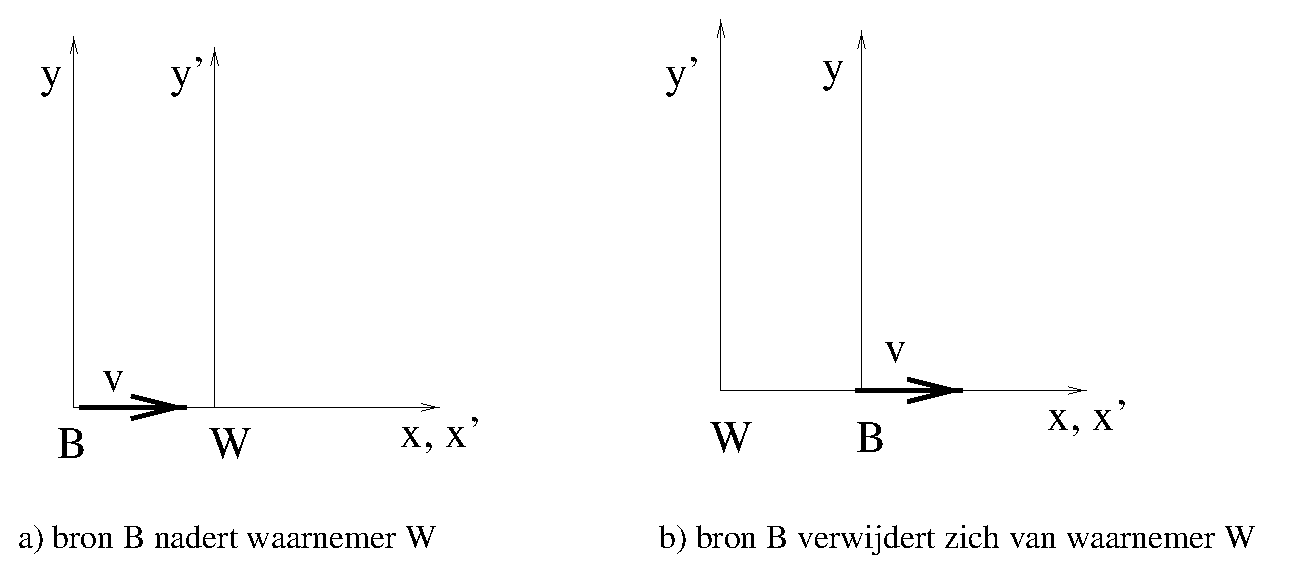
\includegraphics[width=.8\textwidth]{oefeningen.pictures/doppler}
\caption{Bewegende bronnen}
\label{f:doppler}
\end{figure}

We plaatsen een lichtbron in stelsel $S$ en een waarnemer in
stelsel $S'$ met een onderlinge snelheid $v$ tussen $S$ en $S'$.
De Lorentztransformatie geeft dan aan hoe de energie/frequentie, die de 
waarnemer aan de bewegende lichtbron toekent,
afwijkt van de energie/frequentie voor een stilstaande bron.

Eerst: de bron $B$ nadert de waarnemer $W$ (links in fig \ref{f:doppler}a)
\begin{itemize}
\item [a.]
Wat is de Lorentztransformatie voor impuls en energie voor een overgang van
$S$ naar $S'$?
\item [b.]
Leid hieruit de frequentie voor een naderende lichtbron af.
\item [c.]
Ga na of het Doppler-effect hier tot een hogere of lagere frequentie heeft 
geleid.
\end{itemize}
Nu voor een zich verwijderende bron (rechts in figuur \ref{f:doppler}b).
\begin{itemize}
\item [d.]
Bepaal $E'$ en leid de frequentie voor de zich verwijderende bron af.
\item [e.]
Is $\nu '$ groter of kleiner dan $\nu $?
\item [f.]
In welke van de twee gevallen is er sprake van een `roodverschuiving'?
\end{itemize}

%%%%%%%%%%%%%%
\subsection{Roodverschuiving}
In het uitdijend heelal verwijderen veraf gelegen sterrenstelsels zich van ons
af met een snelheid $v$ die toeneemt met hun afstand $d : v \approx Hd$ 
($H$ is de Hubble constante).
Deze verwijdering valt af te lezen uit de `roodverschuiving' van bekende 
spectraallijnen, die nu een grotere golflengte $\lambda '$ dan de 
gebruikelijke $\lambda$ hebben.

De roodverschuiving wordt beschreven door de parameter 
$z = \frac{\lambda ' - \lambda}{\lambda}$.
\begin{itemize}
\item [a.]
Laat zien dat $z = \sqrt{\frac{1 + \beta}{1 - \beta}} -1$.
\item [b.]
Schets een grafiek van $z$ tegen $\beta$.
\end{itemize}
Voor melkwegstelsels op een afstand $d = 10^{8}$   lichtjaar is 
$z \approx 10^{-2}$.
Voor quasars op een afstand $d = 10^{10}$ lichtjaar is $z \approx 1$.
\begin{itemize}
\item [c.]
Maak met deze gegevens een schatting van de Hubble-constante.
\item [d.]
Bereken $\frac{1}{H}$ en laat zien dat deze van de orde van de ouderdom van het heelal is.
\end{itemize}

%%%%%%%%%%%%%%%
\subsection{Stoplicht}
Hoe hard moet je rijden om een stoplicht, dat op rood staat, als een groen
stoplicht te zien?
De golflengte van rood licht is 700 nm, die van groen licht 500 nm.

%%%%%%%%%%%%%%
\subsection{Transversaal Doppler-effect}
In stelsel $S$ staat een waarnemer $W$ ergens op de positieve $y$-as en 
beweegt een lichtbron $B$ zich met snelheid $v$ naar rechts langs 
de $x$-as. We kijken naar de lichtstraal die $B$ in de richting van $W$ 
uitzendt als $B$ op $t=0$ de oorsprong van $S$ passeert (dus een 
foton dat zich langs de positieve $y$-as beweegt, 
met impuls $p_{y}=\frac{E}{c}=\frac{h\nu}{c}$).
\begin{itemize}
\item [a.]
Geef de Lorentztransformatie voor de energie-impuls viervector tussen 
stelsel $S$ en het ruststelsel $S'$ van de lichtbron 
(de stelsels vallen samen op $t=t'=0$).
\item [b.]
Teken de lichtstraal van $B$ naar $W$ in $S'$. Loopt die schuin naar 
{\it linksboven} of naar {\it rechtsboven}?
\item [c.]
In $S$ geldt voor het foton: $p_{x}=0$.
Maak hiervan gebruik om een relatie tussen $E$ en $E'$ voor het foton af te 
leiden en laat zien dat hieruit voor de frequentie van het licht volgt:  
$\nu= \nu '\sqrt{1-\beta ^{2}}$
\item [d.]
In $S'$ wijst de impulsvector van het foton schuin naar linksboven, 
met componenten $p'_{x}$  en  $p'_{y}$.
Laat met de stelling van Pythagoras en de Lorentztransformatie zien dat 
ook in $S'$ geldt:  $|p'|=\frac{E'}{c}$.
\item [e.]
Is er in dit geval sprake van een Doppler-effect (hoewel de lichtbron geen 
snelheidscomponent naar de waarnemer heeft)?
\item [f.]
Is dit `transversale' Doppler-effect groter of kleiner dan het Doppler-effect 
van een naderende of zich verwijderende lichtbron?
\item [g.]
De niet-relativistische Doppler-formule voor een naderende lichtbron is:

\begin{eqnarray}
\nu_{D_{L+}} &=& \frac{c}{c-\nu}\nu = \frac{1}{1-\beta}\nu ;   \\
 \mathrm{en\ }  \nu_{D_T} &=& \nu \  \mathrm{(voor\ 
een\ transversaal\ bewegende\ lichtbron).} \nonumber
\end{eqnarray}

Laat zien dat het relativistische Doppler-effect gelijk is aan het `niet-relativistische Dopper effect gecombineerd met tijddilatatie'.
\end{itemize}



\subsection{Tweelingparadox}
Op Nieuwjaarsdag 2010 vertrekt een astronaut A van de aarde met
snelheid $\beta=0.8$, om naar de dichtsbijzijnde ster, $\alpha$-centauri te gaan. Deze ster staat 4 lichtjaren weg, gemeten in het
coordinatenstelsel verbonden met de aarde. Nadat A de ster heeft
bereikt, keert hij onmiddelijk om en keert terug naar aarde met
dezelfe snelheid, om aan te komen op Nieuwjaarsdag 2020 (aardse
tijd). De astronaut heeft een broer B die achterblijft op aarde, en ze
spreken af elkaar elk jaar op Nieuwjaarsdag een radiobericht te sturen totdat
de reiziger terug is.
\begin{enumerate}
\item Laat zien dat A 6 boodschappen stuurt (inclusief die op de dag van aankomst) terwijl B 10 boodschappen verstuurt.
\item Teken een ruimte-tijd diagram van de reis van A in aardse co\"{o}rdinaten. Teken ook de wereldlijnen van de 
boodschappen die B verstuurd. Laat met dit diagram zien dat A slechts 1 bericht heeft ontvangen op het moment dat hij omkeert,
en dat hij er vervolgens 9 ontvangt tijdens de tweede helft van zijn reis.
\item
Teken een nieuw ruimte-tijd diagram, weer in aardse co\"{o}rdinaten, en teken daarin de wereldlijnen van de astronaut en al de
berichten die {\it hij} verstuurt. Laat zien dat zijn broer op aarde elke 3 jaar een bericht ontvangt gedurende de eerste 9 jaar en dan
3 tijdens het laatste jaar: een totaal van 6.
\item Interpreteer deze resultaten in termen van het Doppler-effect.

\end{enumerate}




					%bijgewerkt 17:02-17/01/2009
% \include{Dynamica}
\section{Deeltjesproductie}

%%%%%%%%
\subsection{Vierimpuls}

% \begin{figure} [h]
% \begin{center}
% \mbox{\epsfxsize=12cm\epsffile{oefeningen.pictures/productie.eps}}
% \caption{}
% \label{f:productie}
% \end{center}
% \end{figure}

\begin{figure}[ht]
\centering
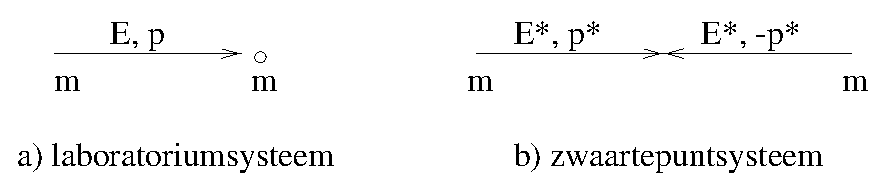
\includegraphics[width=.8\textwidth]{oefeningen.pictures/productie}
\caption{}
\label{f:productie}
\end{figure}

Een deeltje met massa $m$ botst op een zelfde deeltje in 
rust (fig. \ref{f:productie}a).
\begin{itemize}
\item [a.]
Wat is de vierimpuls van een ieder van de deeltjes?
\item [b.]
Wat is de norm van ieder van deze vierimpulsen?
\item [c.]
Wat is de totale vierimpuls in het laboratoriumsysteem?
\end{itemize}
Beschouw nu de botsing in het zwaartepuntsysteem (fig. \ref{f:productie}b).
\begin{itemize}
\item [d.]
Wat is de totale vierimpuls in het zwaartepunt systeem?
\item [e.]
Wat is de norm van deze vierimpuls?
\item [f.]
Vind de uitdrukking voor $E$ in termen van $E^{*}$ en $m$.
\end{itemize}

\subsection{$p\vec{p}$ botsing}
In het zwaartepuntsysteem botsten een
proton (symbool $p$) en een antiproton (symbool $\bar{p}$) ieder met een
snelheid $v= 0,8c$ op elkaar.
De massa van het antiproton is gelijk aan de massa van het proton.
\begin{itemize}
\item [a.]
Wat is de totale impuls $p^{*}$ in het zwaartepuntsysteen?
\item [b.]
Wat is de totale energie $E^{*}$ in het zwaartepuntsysteem?
\item [c.]
Wat is de totale vierimpuls $P^{*}$ in het zwaartepuntsysteem?
\item [d.]
Bij de botsing vernietigen de twee deeltjes elkaar.
Hoeveel energie is er beschikbaar voor de creatie van nieuwe
deeltjes?
\end{itemize}

%%%%%%%%%%%%%
\subsection{Vervallende deeltjes}
Een deeltje in rust met massa $M$ vervalt in twee identieke deeltjes, elk 
met massa $m$.
\begin{itemize}
\item [a.]
Waarom zullen de twee deeltjes die ontstaan een even grote snelheid hebben?
\item [b.]
Geef een uitdrukking voor deze snelheid $v$ in termen van
$M$ en $m$.
\end{itemize}
Een pion (massa $m_{\pi})$ in rust vervalt in een muon (massa $m_{\mu})$ en een
neutrino (massa $m_{\nu} = 0$).
\begin{itemize}
\item [c.]
Wat is de snelheid van het neutrino?
\item [d.]
Wat is de impuls van het muon?
\end{itemize}

%%%%%%%%%%%
\subsection{$pp$ botsing}

% \begin{figure} [h]
% \begin{center}
% \mbox{\epsfxsize=12cm\epsffile{oefeningen.pictures/ppbotsing.eps}}
% \caption{pp botsing}
% \label{f:ppbotsing}
% \end{center}
% \end{figure}

\begin{figure}[ht]
\centering
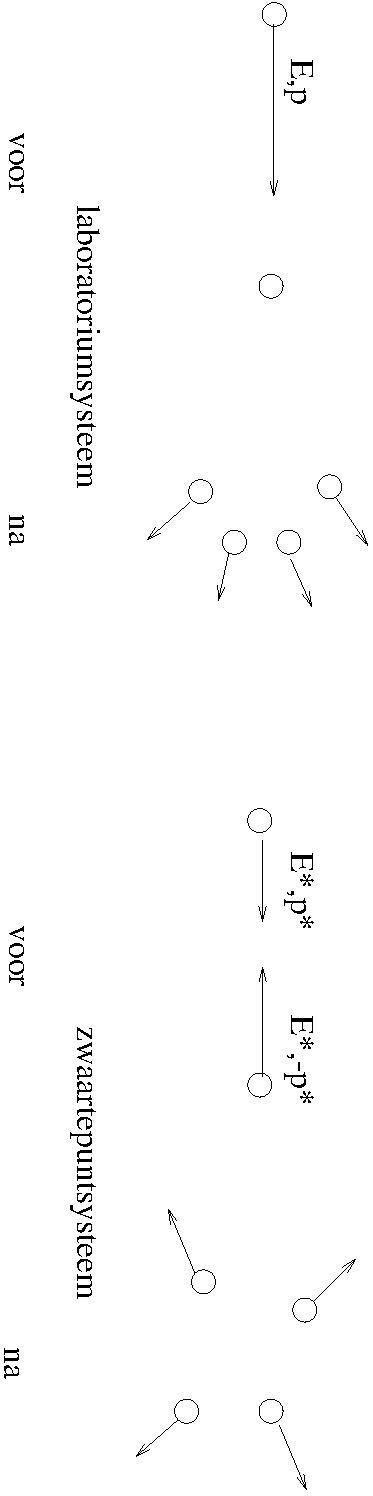
\includegraphics[width=.8\textwidth]{oefeningen.pictures/ppbotsing}
\caption{pp botsing}
\label{f:ppbotsing}
\end{figure}

Wanneer een proton met voldoende energie op een andere proton wordt
geschoten is het mogelijk dat een extra $p\bar{p}$ paar wordt gecre\"{e}erd:
$pp \rightarrow ppp\bar{p}$ 

Bekijk de gebeurtenis eerst vanuit het laboratoriumsysteem
(figuur \ref{f:ppbotsing} links).
De energie en impuls van het bewegende proton in het laboratoriumsysteem 
zijn resp. $E$ en $p$.
\begin{itemize}
\item [a.]
Welk verband bestaat er tussen $E$ en $p$?
\item [b.]
Wat is de totale energie in het laboratoriumsysteem v\'{o}\'{o}r de botsing? 
En de totale impuls? 
\item [c.]
Bekijk nu de gebeurtenis in het zwaartepuntsysteem
(figuur \ref{f:ppbotsing} rechts).
Wat is de minimale energie ($E^{*}_{min}$) nodig om de 
reactie $pp \rightarrow ppp\bar{p}$
te laten verlopen?
\item [d]
Leid uit de invariantie van de vierimpuls de waarde voor de minimale 
energie $E_{min}$ af.
\item [e.]
Wat zou energetisch voordeliger zijn: 
de hierboven beschreven botsing met \'{e}\'{e}n bewegend
en \'{e}\'{e}n stilstaand proton of de situatie waarbij twee bewegende 
protonen op elkaar botsen (bij gelijke onderlinge snelheid)?
\end{itemize}

%%%%%%%%%%%%%%
\subsection{Eenheden}
De energie-eenheden eV (elektronvolt), MeV, GeV, enz., kunnen ook gebruikt 
worden om massa en impuls in uit te drukken: de massa van een electron 
is ongeveer  $m_{e}=0,5$ MeV/c$^{2}$.
\begin{itemize}
\item [a.]
Hoe groot zijn dan $\gamma$  en $v$ voor een elektron met energie  
$E=1$ MeV? 
\item [b.]
Hoe groot is zijn impuls? Welke eenheid gebruik je dan?
\item [c]
De massa van een proton is  $m_{p}=1,0$ GeV/$c^2$ .
Hoeveel energie en impuls heeft een proton met snelheid  $v=0,8\ $ $c$?
\end{itemize}

%%%%%%%%%%%%%
\subsection{$e^{-}e^{+}$ botsing}
Een elektron botst in het laboratoriumsysteem met snelheid $v = 0,8c$ op een
positron in rust.
\begin{itemize}
\item [a.]
Bereken hun totale energie in het laboratoriumsysteen 
($E_{tot} = E_{e^{-}} + E_{e^{+}}$) uitgedrukt in 
de elektron massa $m_{e}$.
\item [b.]
Dezelfde vraag in het zwaartepuntssysteem ($E^{*}_{tot} = E^{*}_{e^{-}} + E^{*}_{e^{+}}$).
\end{itemize}
Bij de botsing vernietigen zij elkaar en ontstaan er, gezien vanuit het 
zwaartepuntsysteem, twee gelijke fotonen die tegengesteld aan elkaar 
wegschieten, elk met een energie $E^{*}_{foton} = h \nu$.
\begin{itemize}
\item [c.]
Waarom moeten het twee fotonen zijn en waarom hebben ze dezelfde frequentie?
\end{itemize}
Als de beweging van de fotonen in het zwaartepuntsysteem loodrecht 
op de richting van het elektron is, kun je met een Lorentztransformatie
de energie van de fotonen in het laboratoriumsysteem bepalen.
\begin{itemize}
\item [d.]
Wat is de frequentie van de fotonen in het laboratoriumsysteem?
\end{itemize}
				%bijgewerkt 17:07-17/01/2009
%
\section{Appendix: Divergentie en Rotatie}
\begin{figure}[hb]

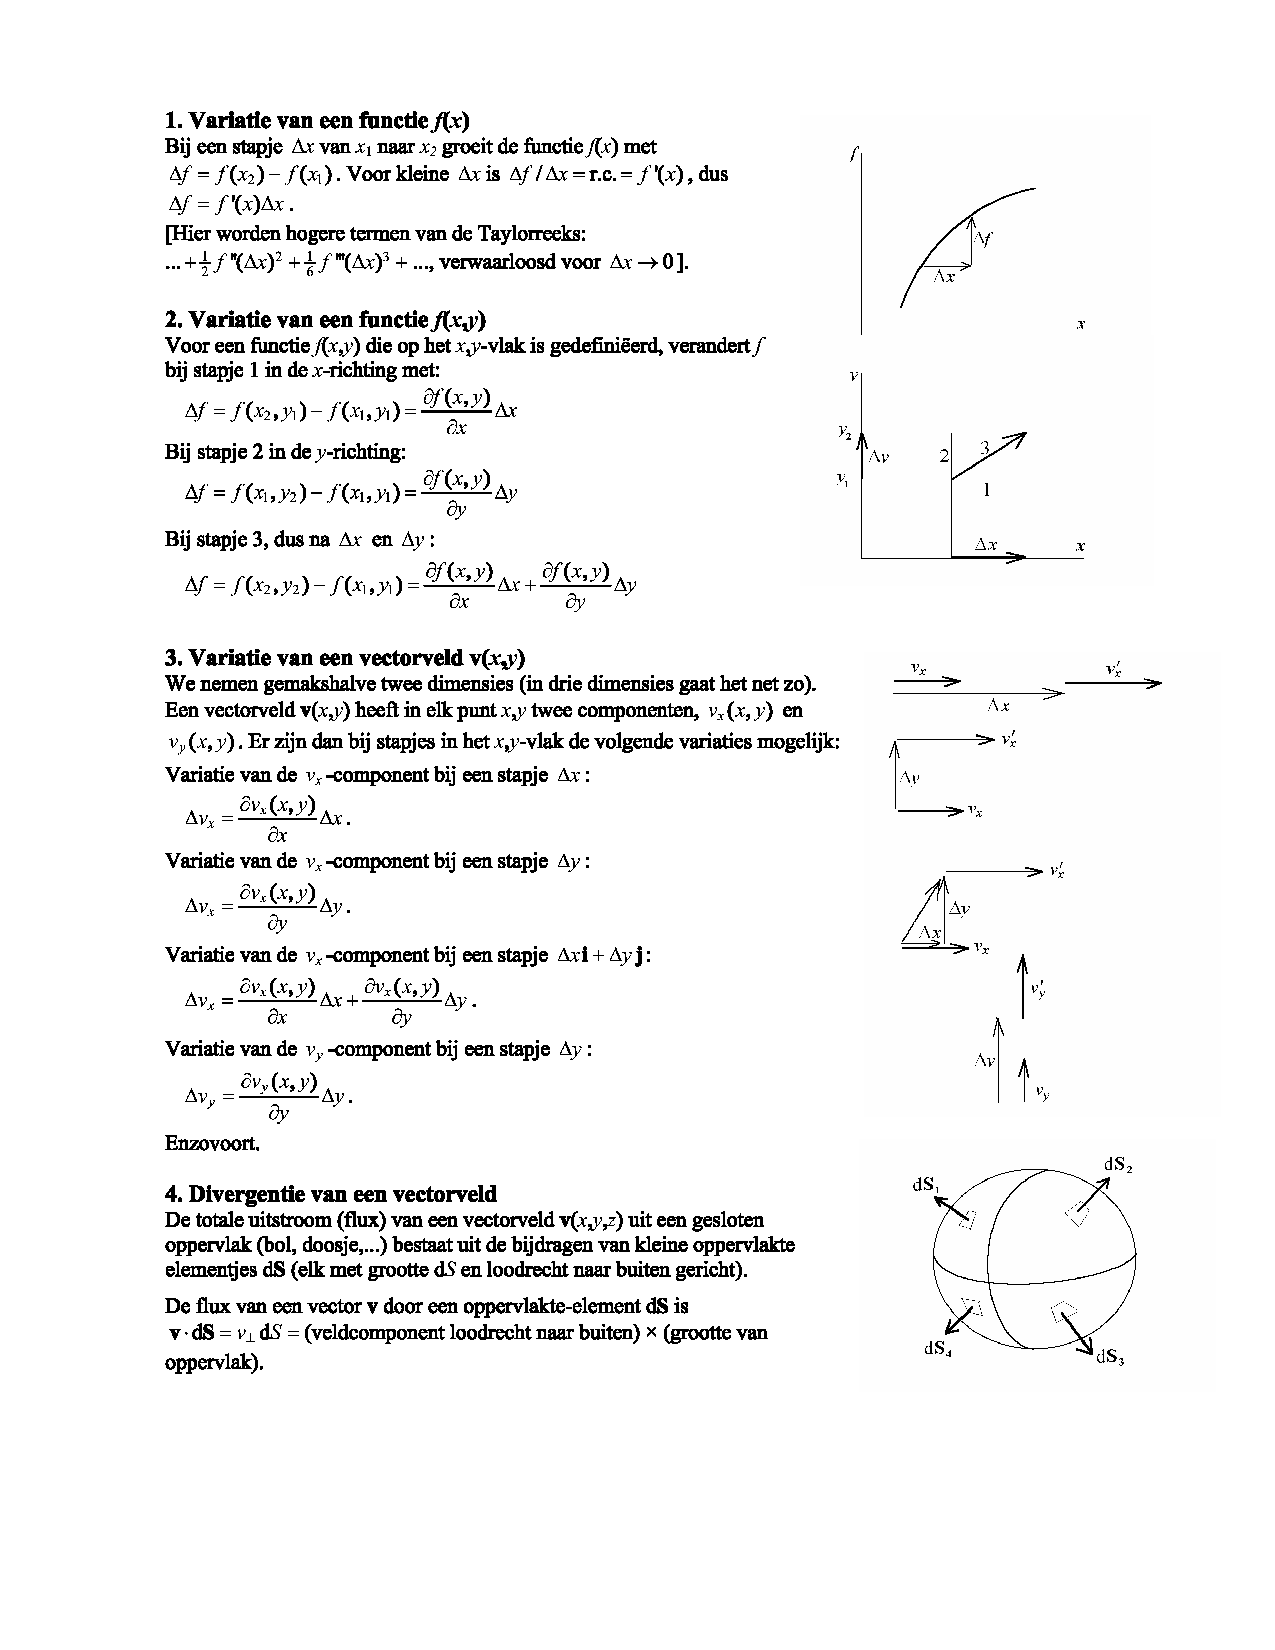
\includegraphics[height=1.00\textwidth]{oefeningen.pictures/Div&Rot-1a}
%\caption{Appendix Divergentie en Rotatie}
\end{figure}
\newpage
\begin{figure}[ht]

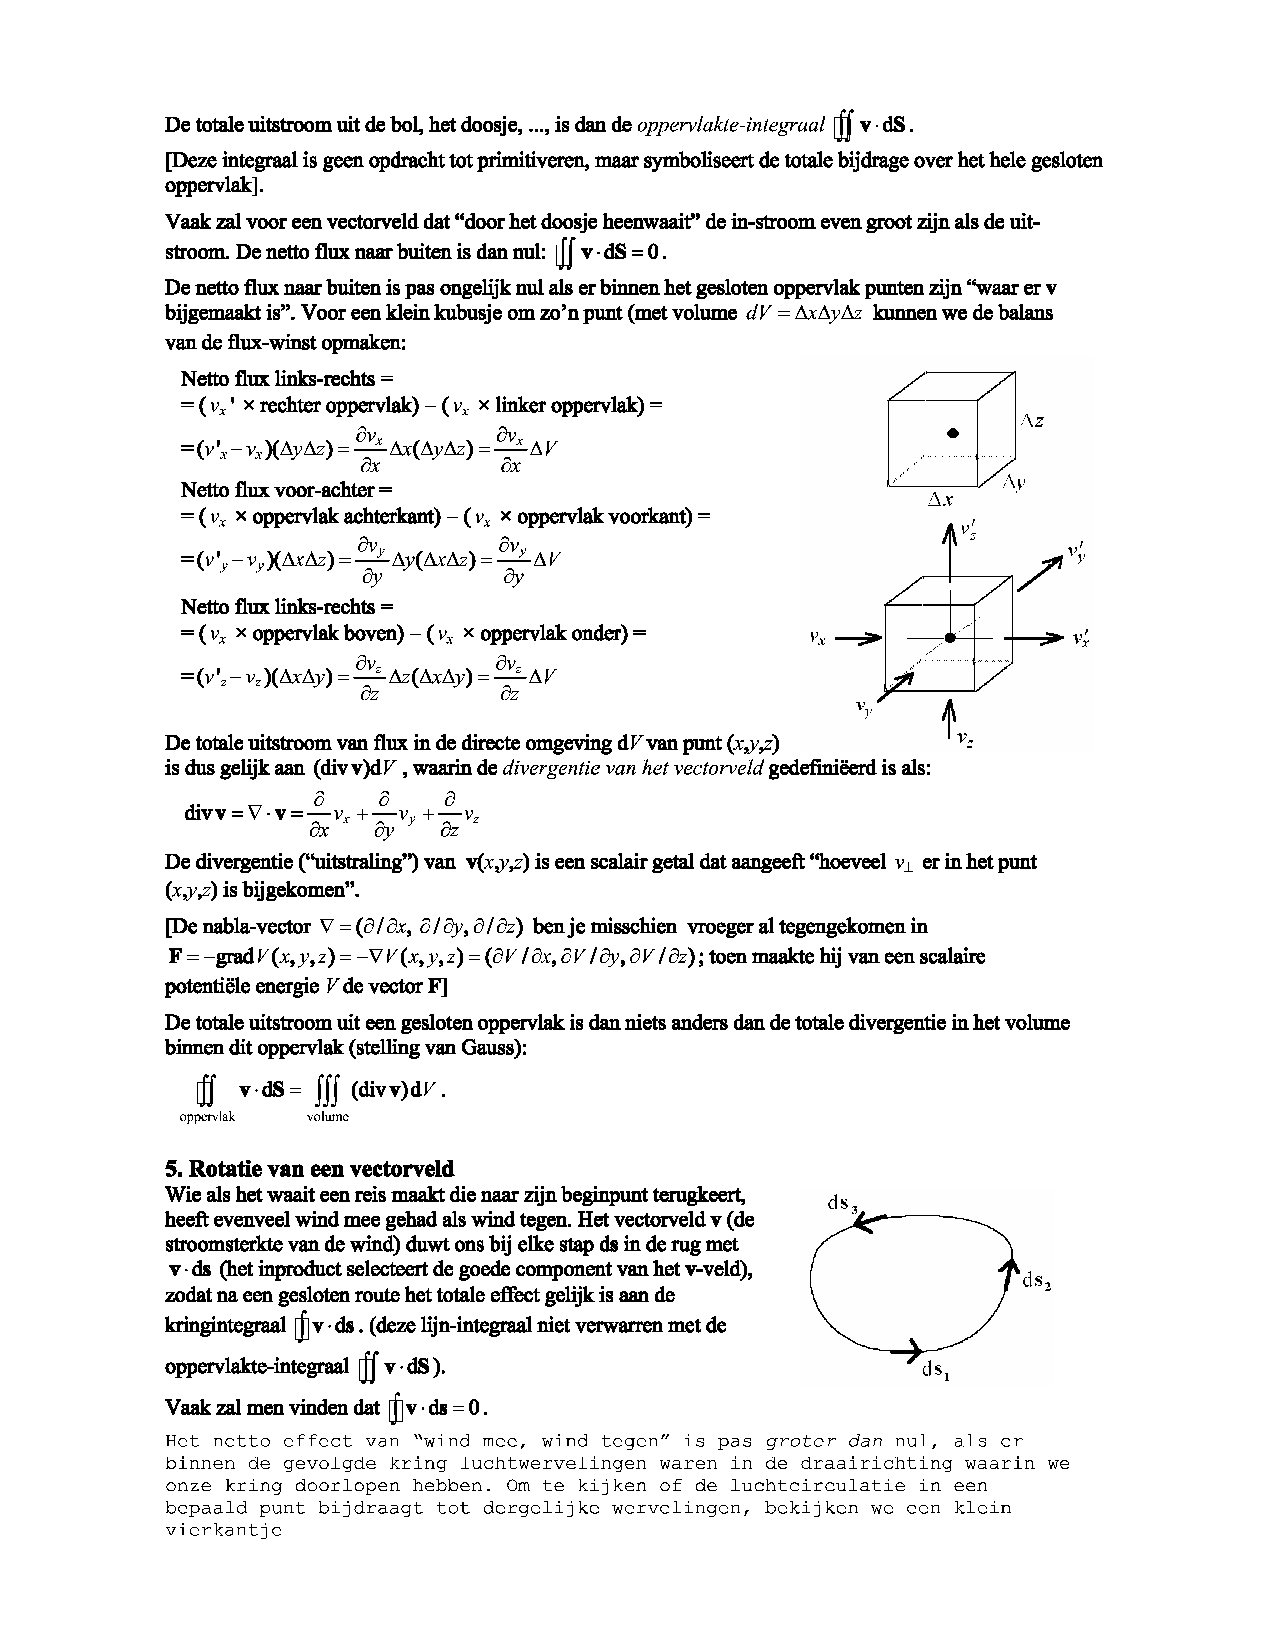
\includegraphics[width=1.0\textwidth]{oefeningen.pictures/Div&Rot-1b}
%\caption{Appendix Divergentie en Rotatie}
\end{figure}
\newpage
\begin{figure}[ht]

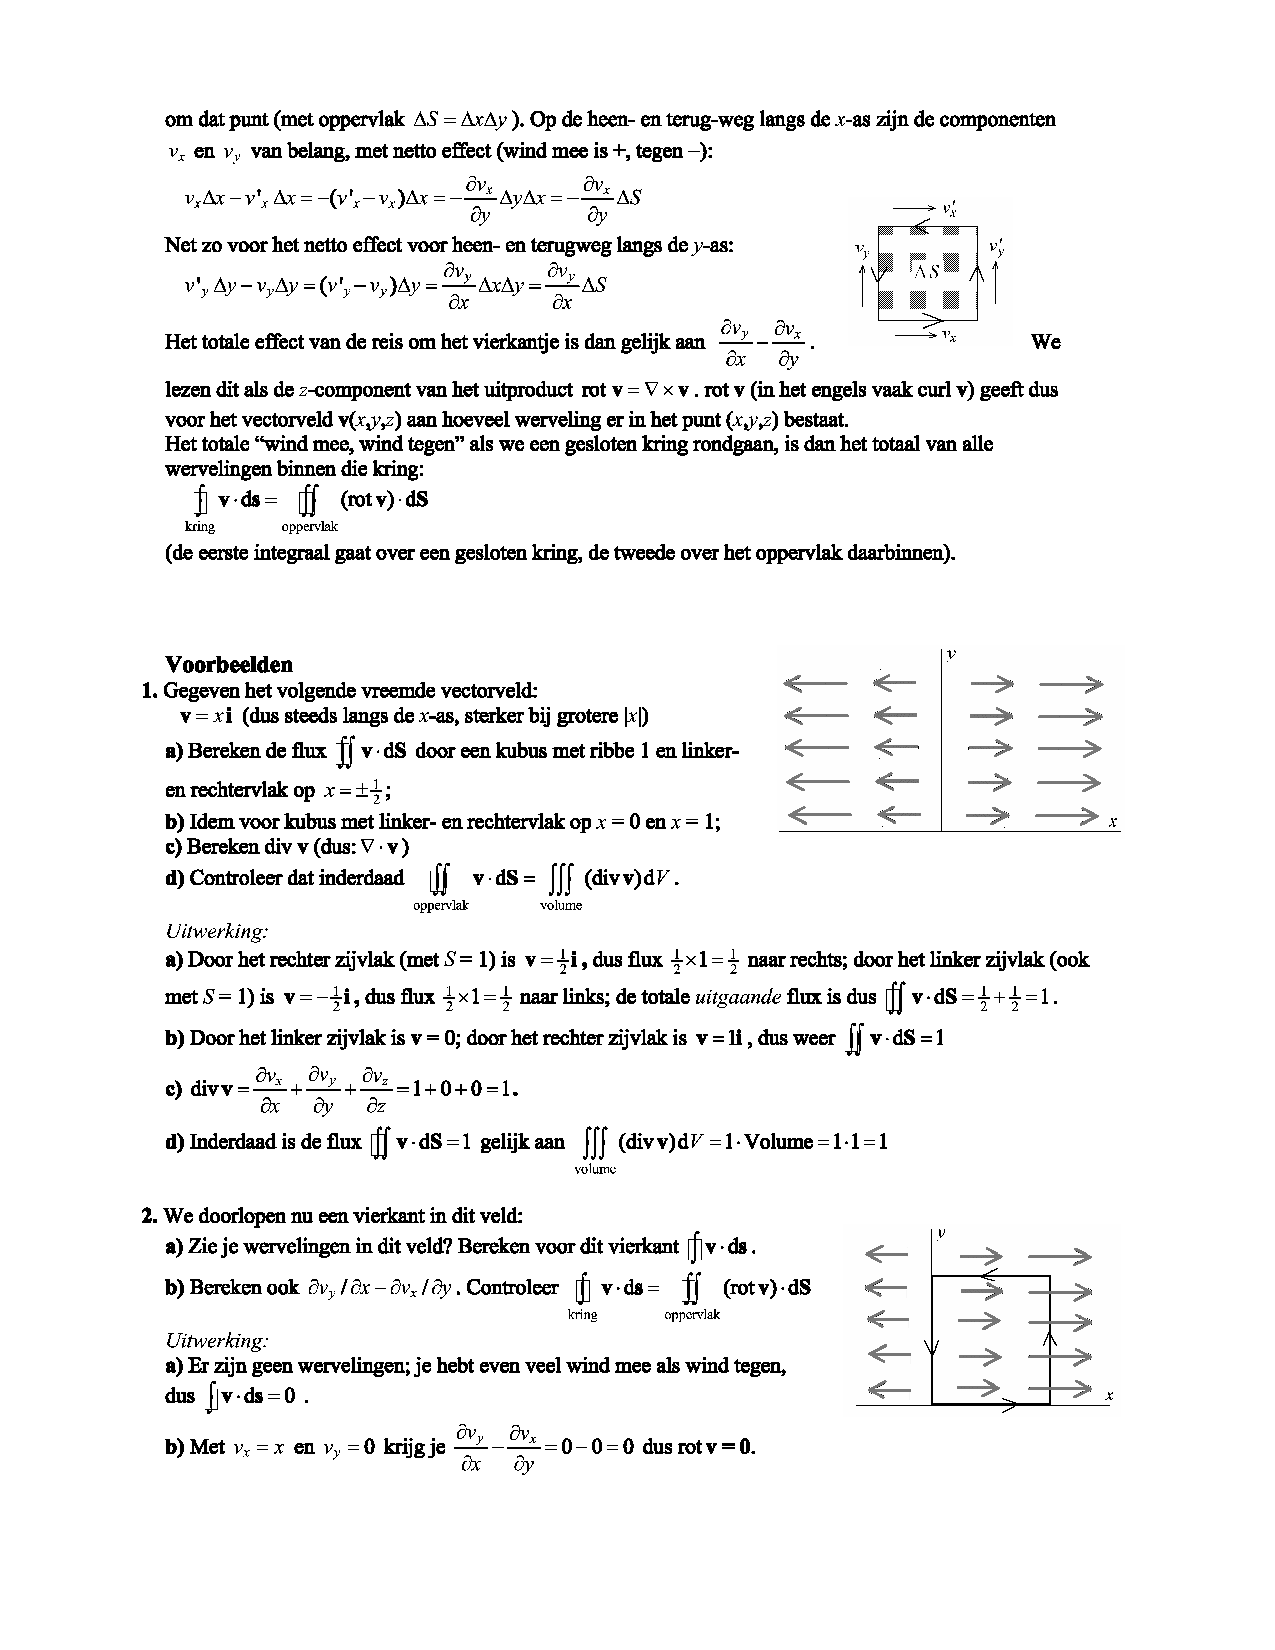
\includegraphics[width=1.0\textwidth]{oefeningen.pictures/Div&Rot-1c}
%\caption{Appendix Divergentie en Rotatie}
\end{figure}
\newpage
\begin{figure}[ht]

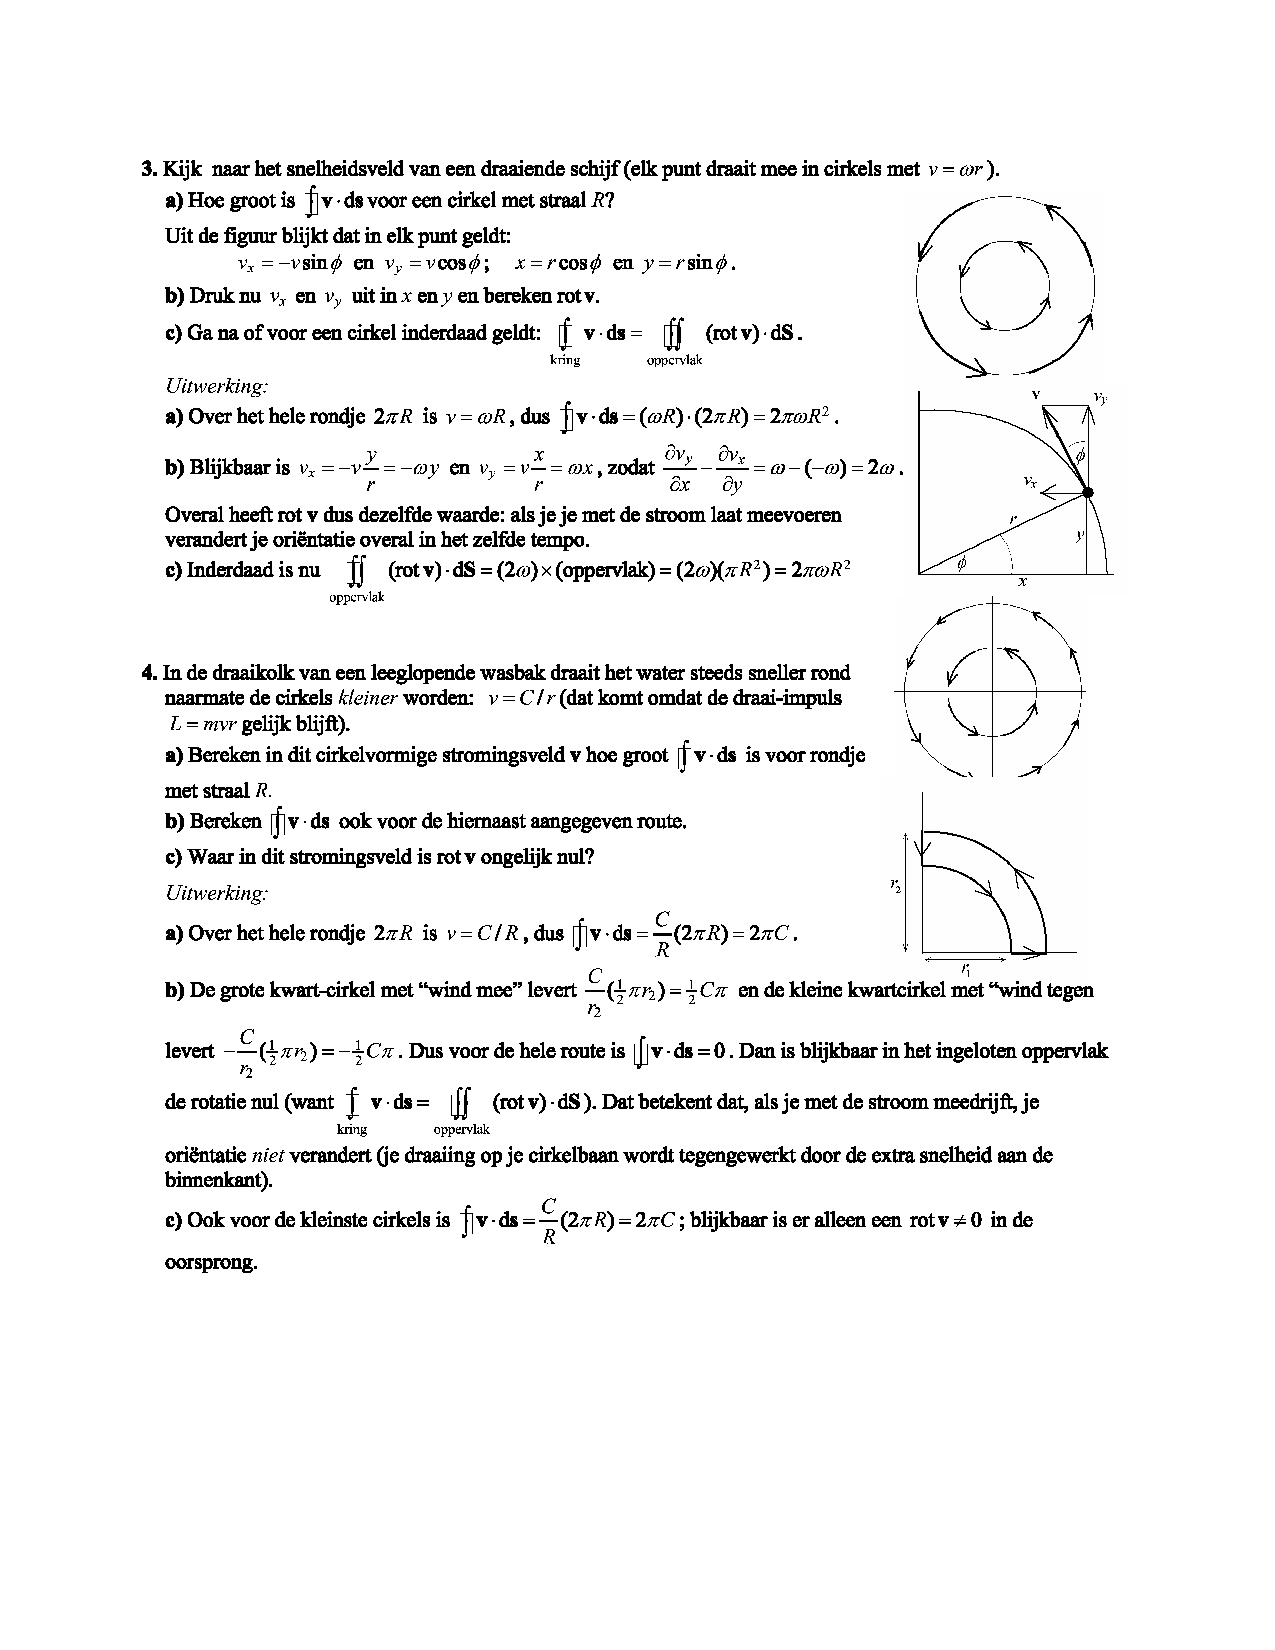
\includegraphics[width=1.0\textwidth]{oefeningen.pictures/Div&Rot-1d}
%\caption{Appendix Divergentie en Rotatie}
\end{figure}
				%in Syllabus_2009
% \include{EM}

\end{document}
